\section{Modelo macroeconométrico}
\label{Modelo_empirico}

\subsection{Investimento residencial e a taxa própria de juros dos imóveis}
\label{SecTxPropria}

O objetivo desta subseção é detalhar a relação entre investimento residencial e a taxa própria de juros dos imóveis desenvolvida por \textcite{teixeira_crescimento_2015} para então expor as hipóteses testadas no modelo econométrico.
Para evidenciar esta relação, deflaciona-se a taxa de juros hipotecária pela inflação de imóveis tal como na equação \ref{tx_Propria} retomada abaixo
$$
g_{I_h} = \phi_0 + \phi_1\cdot own
$$
O gráfico \ref{gZ_Propria} ilustra como  este deflacionamento é mais adequado do que por um índice geral de preços ---  como faz \textcite[p.~143--146]{fair_macroeconometric_2013} --- para captar a dinâmica do investimento residencial.
Destaca-se também que em momentos de bolha de imóveis é a inflação destes ativos que domina a dinâmica da taxa própria \cite[p.~53]{teixeira_crescimento_2015}. Sendo assim, quanto menor esta taxa maiores serão os ganhos de capital (em imóveis) por se especular com imóveis.
Tal dinâmica é evidenciada no gráfico \ref{gZ_Propria} em que a taxa própria se reduziu progressivamente ao longo do \textit{boom} imobiliário (2002-5).


%TODO Alterar imagem


\begin{figure}[H]
	\centering
	\caption{Taxa de juros hipotecária deflacionada pelo índice de preços ao consumidor e taxa própria de juros dos imóveis x investimento residencial (1987-2019, média móvel trimestral)}
	\label{gZ_Propria}
	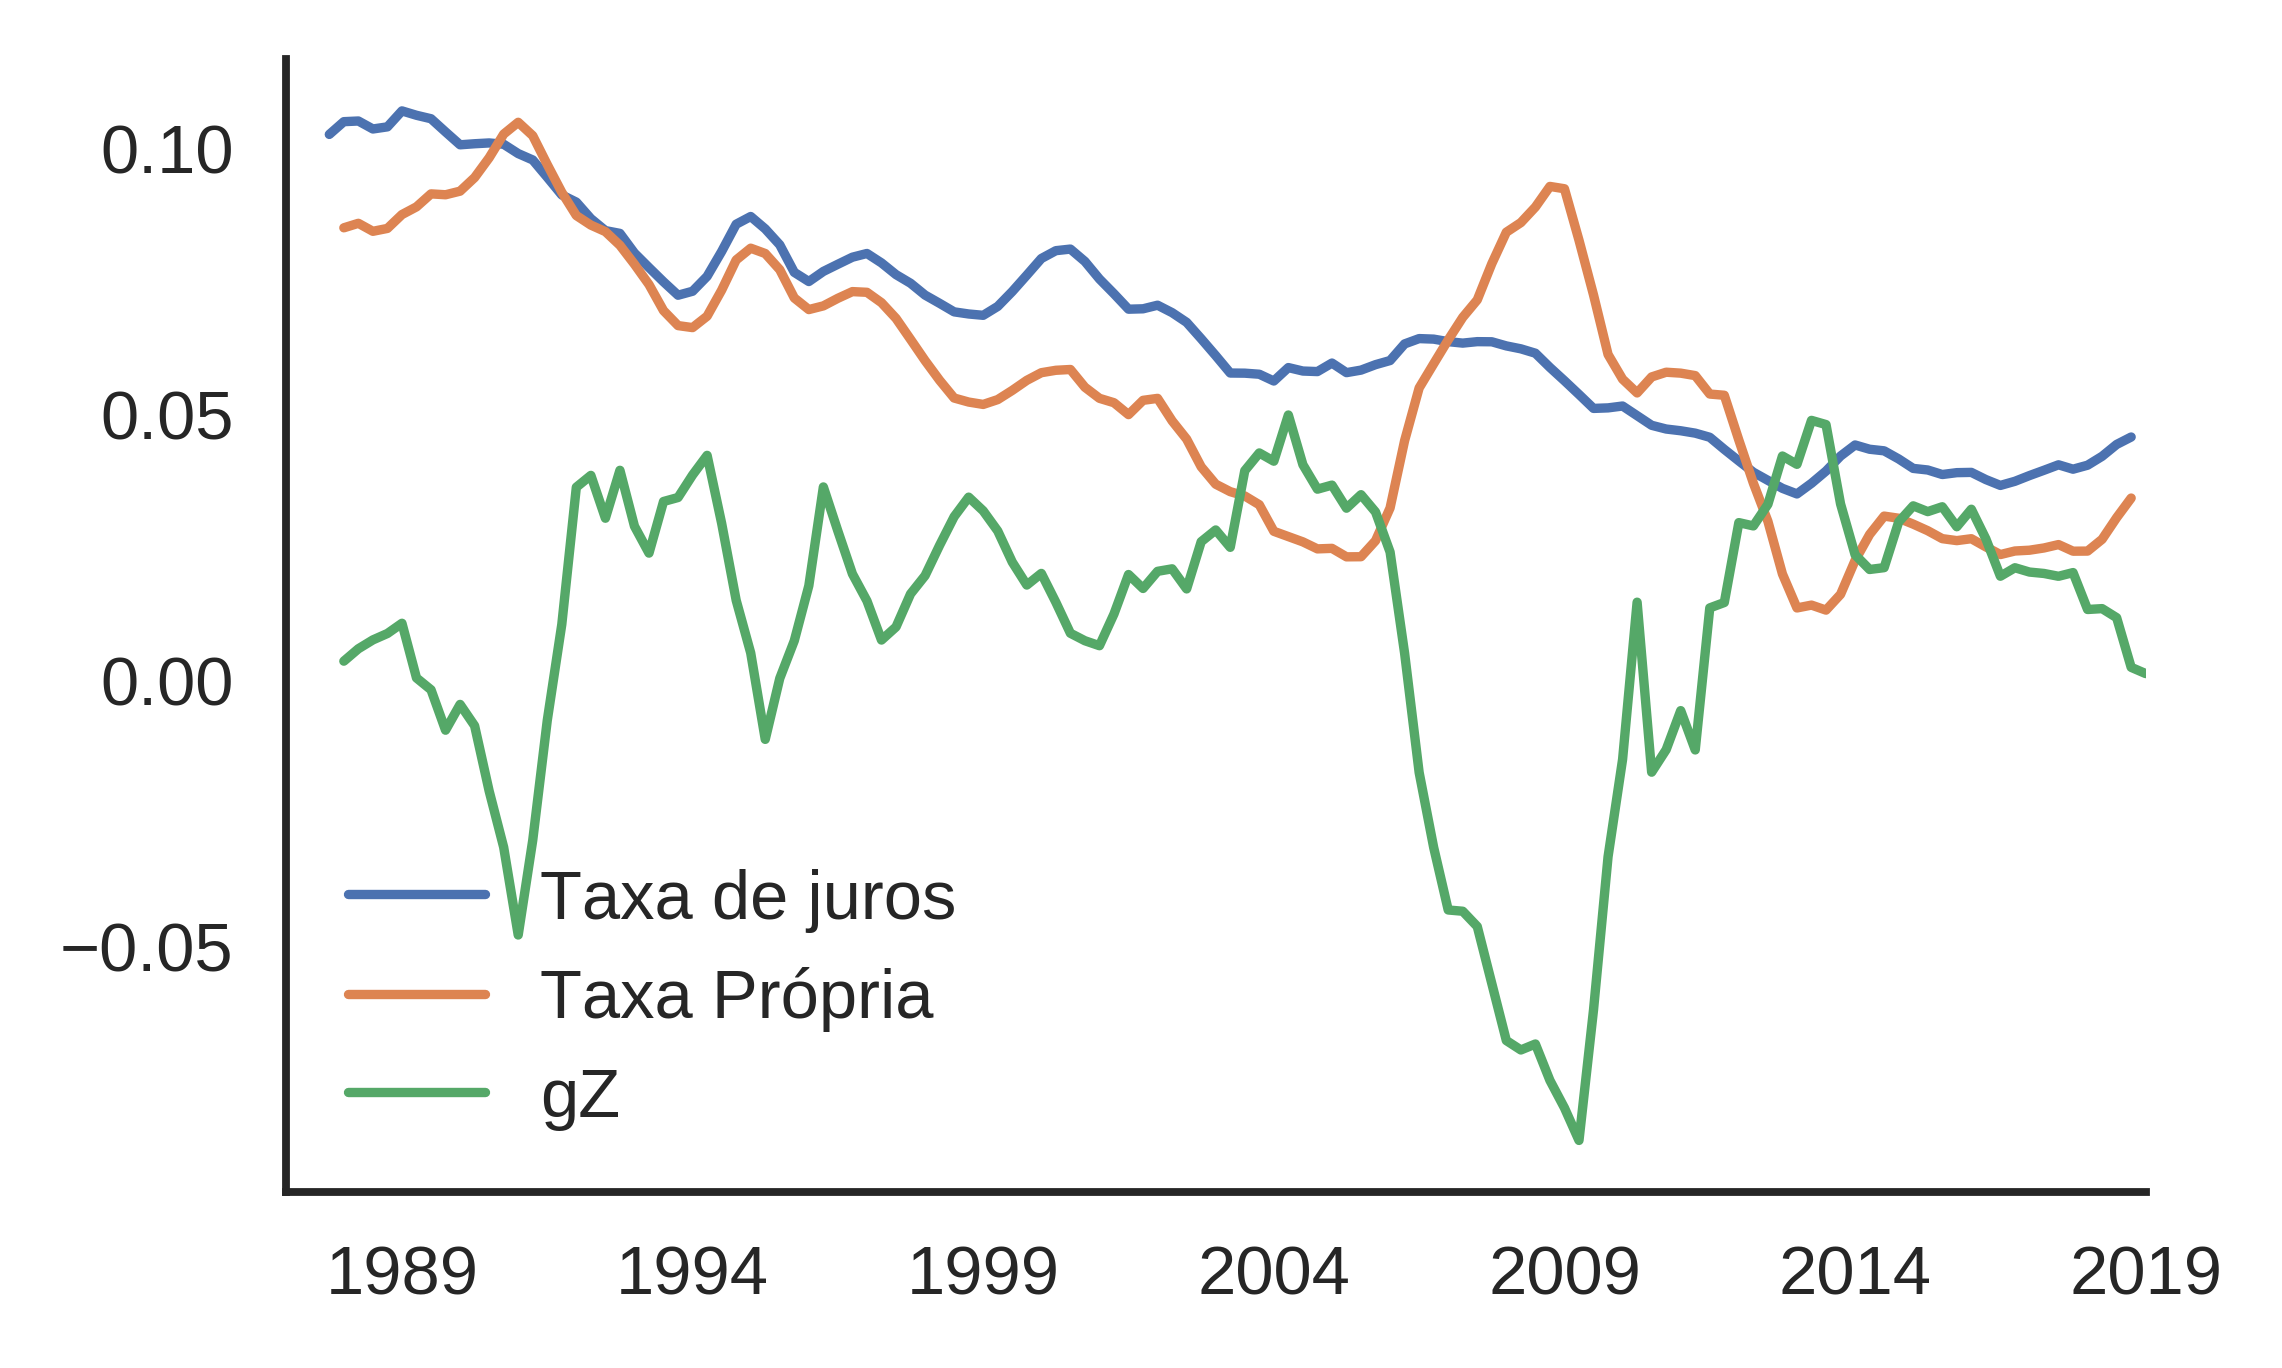
\includegraphics[width=0.75\textwidth]{../../Dados/Fatos_Estilizados/figs/TxPropria_Investo.png}
	\caption*{\textbf{Fonte:} U.S. Bureau of Economic Analysis, elaboração própria}
\end{figure}

De modo a testar a capacidade explicativa da taxa própria para o investimento residencial, assume-se a seguinte relação de longo prazo tal como em \textcite{teixeira_crescimento_2015}:

\begin{equation}
g_{I_{h_t}} = \phi_0 - \phi_1\cdot own_t
\end{equation}
sendo assim, se as séries forem cointegradas, é possível estimar um VECM nos seguintes termos:
\begin{equation}
\begin{cases}
\Delta own_t = \delta_{1} + \alpha_1(g_{I_{h_{t-1}}} - \phi_0 + \phi_1\cdot own_{t-1}) + \sum^{N=4}_{i=1}\beta_{1,i}\cdot \Delta g_{I_{h_{t-i}}} +
\sum^{N=4}_{i=1}\gamma_{1,i}\cdot \Delta own_{t-i} +\varepsilon_{t,1}
\\
\Delta g_{Z_{t}} = \delta_{2} + \alpha_2(g_{I_{h_{t-1}}} - \phi_0 + \phi_1\cdot own_{t-1}) + \sum^{N=4}_{i=1}\beta_{2,i}\cdot \Delta g_{I_{h_{t-i}}} +
\sum^{N=4}_{i=1}\gamma_{2,i}\cdot \Delta own_{t-i} +\varepsilon_{t,2}
\end{cases}
\end{equation}
em que $\delta_s$ indicam tendência linear nas respectivas séries em nível;
$\alpha_{is}$ são os coeficientes de correção de erro; 
$\beta_s$ e $\gamma_s$ são coeficientes associados as defasagens de  $g_{I_h}$ e $own$ respectivamente e; $\varepsilon_s$ são os resíduos.
Seguindo as hipóteses de \textcite{teixeira_crescimento_2015}, os resultados esperados a serem testados estão na tabela \ref{resultados_esperados} abaixo:


% Please add the following required packages to your document preamble:
% \usepackage{graphicx}
\begin{table}[H]
	\centering
	\caption{Resumo dos resultados esperados do modelo macroeconométrico}
	\label{resultados_esperados}
	\resizebox{\textwidth}{!}{%
		\begin{tabular}{l|l|l}
			\hline\hline
			\textbf{\begin{tabular}[c]{@{}l@{}}Resultado\\ Esperado\end{tabular}} &
			\textbf{Significado econométrico} &
			\textbf{Significado econômico} \\ \hline\hline
			\textbf{1. $\varepsilon \sim I(0)$} &
			\begin{tabular}[c]{@{}l@{}}Estacionariedade dos resíduos indica cointegração\end{tabular} &
			\begin{tabular}[c]{@{}l@{}}Séries apresentam uma dinâmica \\ de longo prazo em comum\end{tabular} \\ \hline
			\textbf{2. $\alpha_1 = 0$} &
			\begin{tabular}[c]{@{}l@{}}Variável $own$ exogenamente\\ fraca em relação a $g_{I_h}$\end{tabular} & \begin{tabular}[c]{@{}l@{}} O comportamento dinâmico de $own$ não\\é afetado pelo desvio do equilíbrio no período anterior\end{tabular}
			\\ \hline
			\textbf{3. $\alpha_2 < 0$} &
			\begin{tabular}[c]{@{}l@{}}Taxa própria causa (no sentido de Granger)\\ a taxa de crescimento do investimento residencial\end{tabular} & \begin{tabular}[c]{@{}l@{}} O comportamento dinâmico de $g_{I_h}$ é\\ afetado pelo desvio do equilíbrio no período anterior\end{tabular}
			\\ \hline
			\textbf{4. $\phi_1 > 0$} &
			\begin{tabular}[c]{@{}l@{}}Séries apresentam uma dinâmica\\ negativa no longo prazo\end{tabular} &
			\begin{tabular}[c]{@{}l@{}}Taxa própria afeta taxa de crescimento\\ do investimento residencial negativamente\end{tabular} \\ \hline
			\textbf{5. $\phi_0 < 0$} &
			\begin{tabular}[c]{@{}l@{}}Coeficiente associado a demanda por\\ imóveis por motivos não especulativos é\\ estatistacamente significante\end{tabular} &
			\begin{tabular}[c]{@{}l@{}}Taxa de crescimento do investimento residencial\\ é determinada positivamente pela demanda por \\ imóveis associada a especificidades institucionais e\\ mudanças demográficas\end{tabular} \\ \hline
			\textbf{6. $\gamma_{2,is} < 0$} &
			\begin{tabular}[c]{@{}l@{}}Coeficiente associado a taxa de crescimento\\ do investimento residencial é estatisticamente\\ significante\end{tabular} &
			\begin{tabular}[c]{@{}l@{}}Taxa própria afeta a taxa de crescimento do investimento\\ residencial negativamente no curto prazo\end{tabular} \\ \hline
			\textbf{7. $\beta_{1,is} = 0$} &
			\begin{tabular}[c]{@{}l@{}}Efeito do investimento de $g_{I_h}$ sobre a \\ taxa própria não é estatisticamente significante\end{tabular} &
			\begin{tabular}[c]{@{}l@{}}Efeito da taxa de crescimento do investimento residencial sobre\\ o preço dos imóveis é desprezível dado que o estoque de imóveis\\ é muito maior que o fluxo de novos imóveis\end{tabular} \\ \hline\hline
		\end{tabular}%
	}
\end{table}

Apesar de lançar luz sobre algumas relações relevantes, a proposição de \textcite{teixeira_crescimento_2015} não foi avaliada por meio da estimação de um modelo macroeconométrico e isso será feito a seguir.

\subsection{Estimação do modelo}

O modelo a ser estimado pretende testar se a inflação de ativos (\textit{i.e.} inflação do preço dos imóveis) contribui para explicar a dinâmica do investimento residencial tal como proposto por \textcite{teixeira_crescimento_2015}\footnote{Os resultados de todos os testes realizados bem como as rotinas utilizadas estão disponíveis sob solicitação.}. 
Vale relembrar que a seleção do período analisado decorre de quebras estruturais (ver tabela \ref{structbreak}) associadas às mudanças institucionais no-pós crise das \textit{savings and loans} (FDIC e FIRREA).
Dito isso, foram utilizadas séries trimestrais com ajuste sazonal de 1992 a 2019 (ver gráfico \ref{YeoJhonson}) da taxa de juros das hipotecas fixas em trinta anos (MORTGAGE30US, trimestralizada pelo fim do período), investimento residencial (PRFI, em taxa de crescimento) e índice de Case-Shiller (CSUSHPISA, trimestralizada pelo fim do período). 

Por se tratar de taxas de crescimento com ampla volatilidade, aplicou-se a transformação de \textcite{yeo_new_2000} para conter a amplitude das séries decorrente da crise imobiliária. A razão de se utilizar tal procedimento e não a transformação de \textcite{box_analysis_1964} é por não se restringir a valores não-negativos. Em seguida, foram realizados testes de raiz unitária (tabela \ref{unitroot}) bem como o procedimento de \textcite{johansen_estimation_1991} (tabela \ref{Johansen}) e, a um nível de significância de 5\%, conclui-se que as séries são cointegradas e, portanto, um modelo do tipo vetor de correção de erros (VECM) é a melhor forma de estimação para este caso \cite{enders_applied_2014}.


% Please add the following required packages to your document preamble:
% \usepackage{multirow}
% \usepackage{graphicx}
\begin{table}[htb]
	\centering
	\caption{Teste de quebra estrutural}
	\label{structbreak}
	\begin{threeparttable}
	%\resizebox{\textwidth}{!}{%
		\begin{tabular}{l|l|cc}
			\hline \hline
			\multirow{2}{*}{\textbf{Variável}} & \multirow{2}{*}{\textbf{Quebra}} & \multicolumn{2}{c}{\textbf{Teste de Chow}\tnote{a}} \\ \cline{3-4} 
			&& Estatística & p-valor \\ \hline
			\multirow{3}{*}{\textbf{Investimento residencial ($g_{I_h}$)}} & 1991/Q3 & 5.1147 & 0.0254 \\
			& 2005/Q4 & 7.286 & 0.007881 \\
			& 2010/Q3 & 6.1013 & 0.01481 \\ \hline
			\multirow{5}{*}{\textbf{Taxa Própria}} & 1991/Q3 & 63.453 & 7.487e-13 \\
			& 1996/Q3 & 107.47 & \textless 2.2e-16 \\
			& 2001/Q2 & 78.378 & 5.662e-15 \\
			& 2006/Q1 & 20.68 & 1.236e-05 \\
			& 2011/Q1 & 78.969 & 4.663e-15 \\ \hline
			\multirow{4}{*}{\textbf{Taxa de juros das hipotecas}} & 1991/Q3 & 124.35 & \textless 2.2e-16 \\
			& 1997/Q1 & 199.25 & \textless 2.2e-16 \\
			& 2002/Q1 & 301.18 & \textless 2.2e-16 \\
			& 2009/Q4 & 172.97 & \textless 2.2e-16 \\ \hline
			\multirow{3}{*}{\textbf{Inflação de imóveis}} & 1997/Q3 & 1.5508 & 0.2153 \\
			& 2005/Q4 & 23.49 & 3.569e-06 \\
			& 2011/Q3 & 4.4981 & 0.03586 \\ 
			\hline \hline
		\end{tabular}%
	%}
	\begin{tablenotes}\footnotesize
		\item [a] H0: Não há quebra estrutural.
	\end{tablenotes}
\end{threeparttable}
	\caption*{\textbf{Fonte:} Elaboração própria}
\end{table}


% Please add the following required packages to your document preamble:
% \usepackage{multirow}
% \usepackage{graphicx}
\begin{table}[htb]
	\centering
	\caption{Testes de raiz unitária}
	\label{unitroot}
	\resizebox{\textwidth}{!}{%
	\begin{threeparttable}
		\begin{tabular}{l|l|cccccccc}
\hline\hline
\multicolumn{2}{l|}{\multirow{2}{*}{\textbf{Variável}}} & \multicolumn{2}{c}{\textbf{ADF}\tnote{a}} & \multicolumn{2}{c}{\textbf{Zivot Andrews}\tnote{b}} & \multicolumn{2}{c}{\textbf{Phillips Perron}\tnote{a}} & \multicolumn{2}{c}{\textbf{KPSS}\tnote{c}} \\ \cline{3-10} 
\multicolumn{2}{l|}{} & \multicolumn{1}{l}{Estatística} & \multicolumn{1}{l}{p-valor} & \multicolumn{1}{l}{Estatística} & \multicolumn{1}{l}{p-valor} & \multicolumn{1}{l}{Estatística} & \multicolumn{1}{l}{p-valor} & \multicolumn{1}{l}{Estatística} & \multicolumn{1}{l}{p-valor} \\ \hline
\textbf{Investimento} & original &-3.333&0.013&-4.439&0.139&-6.165&0.000&0.181&0.309\\
\textbf{residencial ($g_{I_h}$)} & em diferença &-7.155&0.000&-7.739&0.000&-20.346&0.000&0.106&0.558\\ \hline
\textbf{Inflação} & original &-2.671&0.079&-4.871&0.043&-2.704&0.073&0.148&0.395 \\
\textbf{de imóveis} & em diferença &-4.680&0.000&-6.122&0.001&-11.340&0.000&0.059&0.819 \\ \hline
\textbf{Taxa Própria de juros} & original &-2.330&0.162&-4.203&0.237&-2.425&0.135&0.690&0.014 \\
\textbf{dos imóveis}& em diferença &-5.087&0.000&-6.340&0.000&-10.408&0.000&0.062&0.804\\ \hline
\textbf{Taxa de juros} & original &-3.638&0.027&-4.494&0.215&-3.604&0.030&0.081&0.264 \\
\textbf{das hipotecas}& em diferença &-8.050&0.000&-8.144&0.000&-11.127&0.000 &0.034&0.962 \\ 
\hline\hline
\end{tabular}%
\begin{tablenotes}\footnotesize
	\item [a] H0: presença de raiz unitária.
	\item [b] H0: presença de raiz unitária e de uma quebra estrutural.
	\item [c] H0: série fracamente estacionária.
\end{tablenotes}
\end{threeparttable}
	}
\caption*{\textbf{Fonte:} Elaboração própria}
\end{table}


% Please add the following required packages to your document preamble:
% \usepackage{multirow}
% \usepackage{graphicx}
\begin{table}[htb]
\centering
\caption{Teste de cointegração}
\label{Johansen}
\begin{threeparttable}
%\resizebox{\textwidth}{!}{%
\begin{tabular}{l|l|cc}
\hline
 \hline
\multirow{2}{*}{\textbf{Modelo}} & \multirow{2}{*}{\textbf{Hipótese}\tnote{a}} & \multicolumn{2}{c}{\textbf{Procedimento de Johansen}} \\ \cline{3-4} 
 &  & \multicolumn{1}{c|}{Estatística} & valor crítico (5\%) \\ \hline
\multirow{3}{*}{\textbf{$g_Z$, Taxa Própria}\tnote{b}} & $r = 0$ &20.13&19.96\\
 & $r = 1^*$ &3.57&9.24\\\hline	
\multirow{4}{*}{\textbf{$g_Z$, Inflação e Juros}\tnote{c}} & $r = 0$ &44.34&34.91\\
 & $r = 1$ &26.22&19.96\\
 & $r = 2$ &10.69&9.24\\\hline
\multirow{3}{*}{\textbf{$g_Z$, Inflação e Juros exógeno}\tnote{d}} & $r = 0$ &33.64& 19.96\\ 
 & $r = 1$ &14.03&9.24\\ 
  \hline
\end{tabular}%
%}
\footnotesize{(a) Utilizado teste do traço com constante e defasagem selecionada a partir do critério AIC. (b) Testado para o lag 5. (c) Testado para o lag 5. (d) Testado para o lag 5. (*) Indica que o \textit{rank} selecionado implica em cointegração.}
\end{threeparttable}
\caption*{\textbf{Fonte:} Elaboração Própria}
\end{table}

%TODO Alterar figura
\begin{figure}[htb]
	\centering
	\caption{Séries com transformação de \textcite{yeo_new_2000}}
	\label{YeoJhonson}
	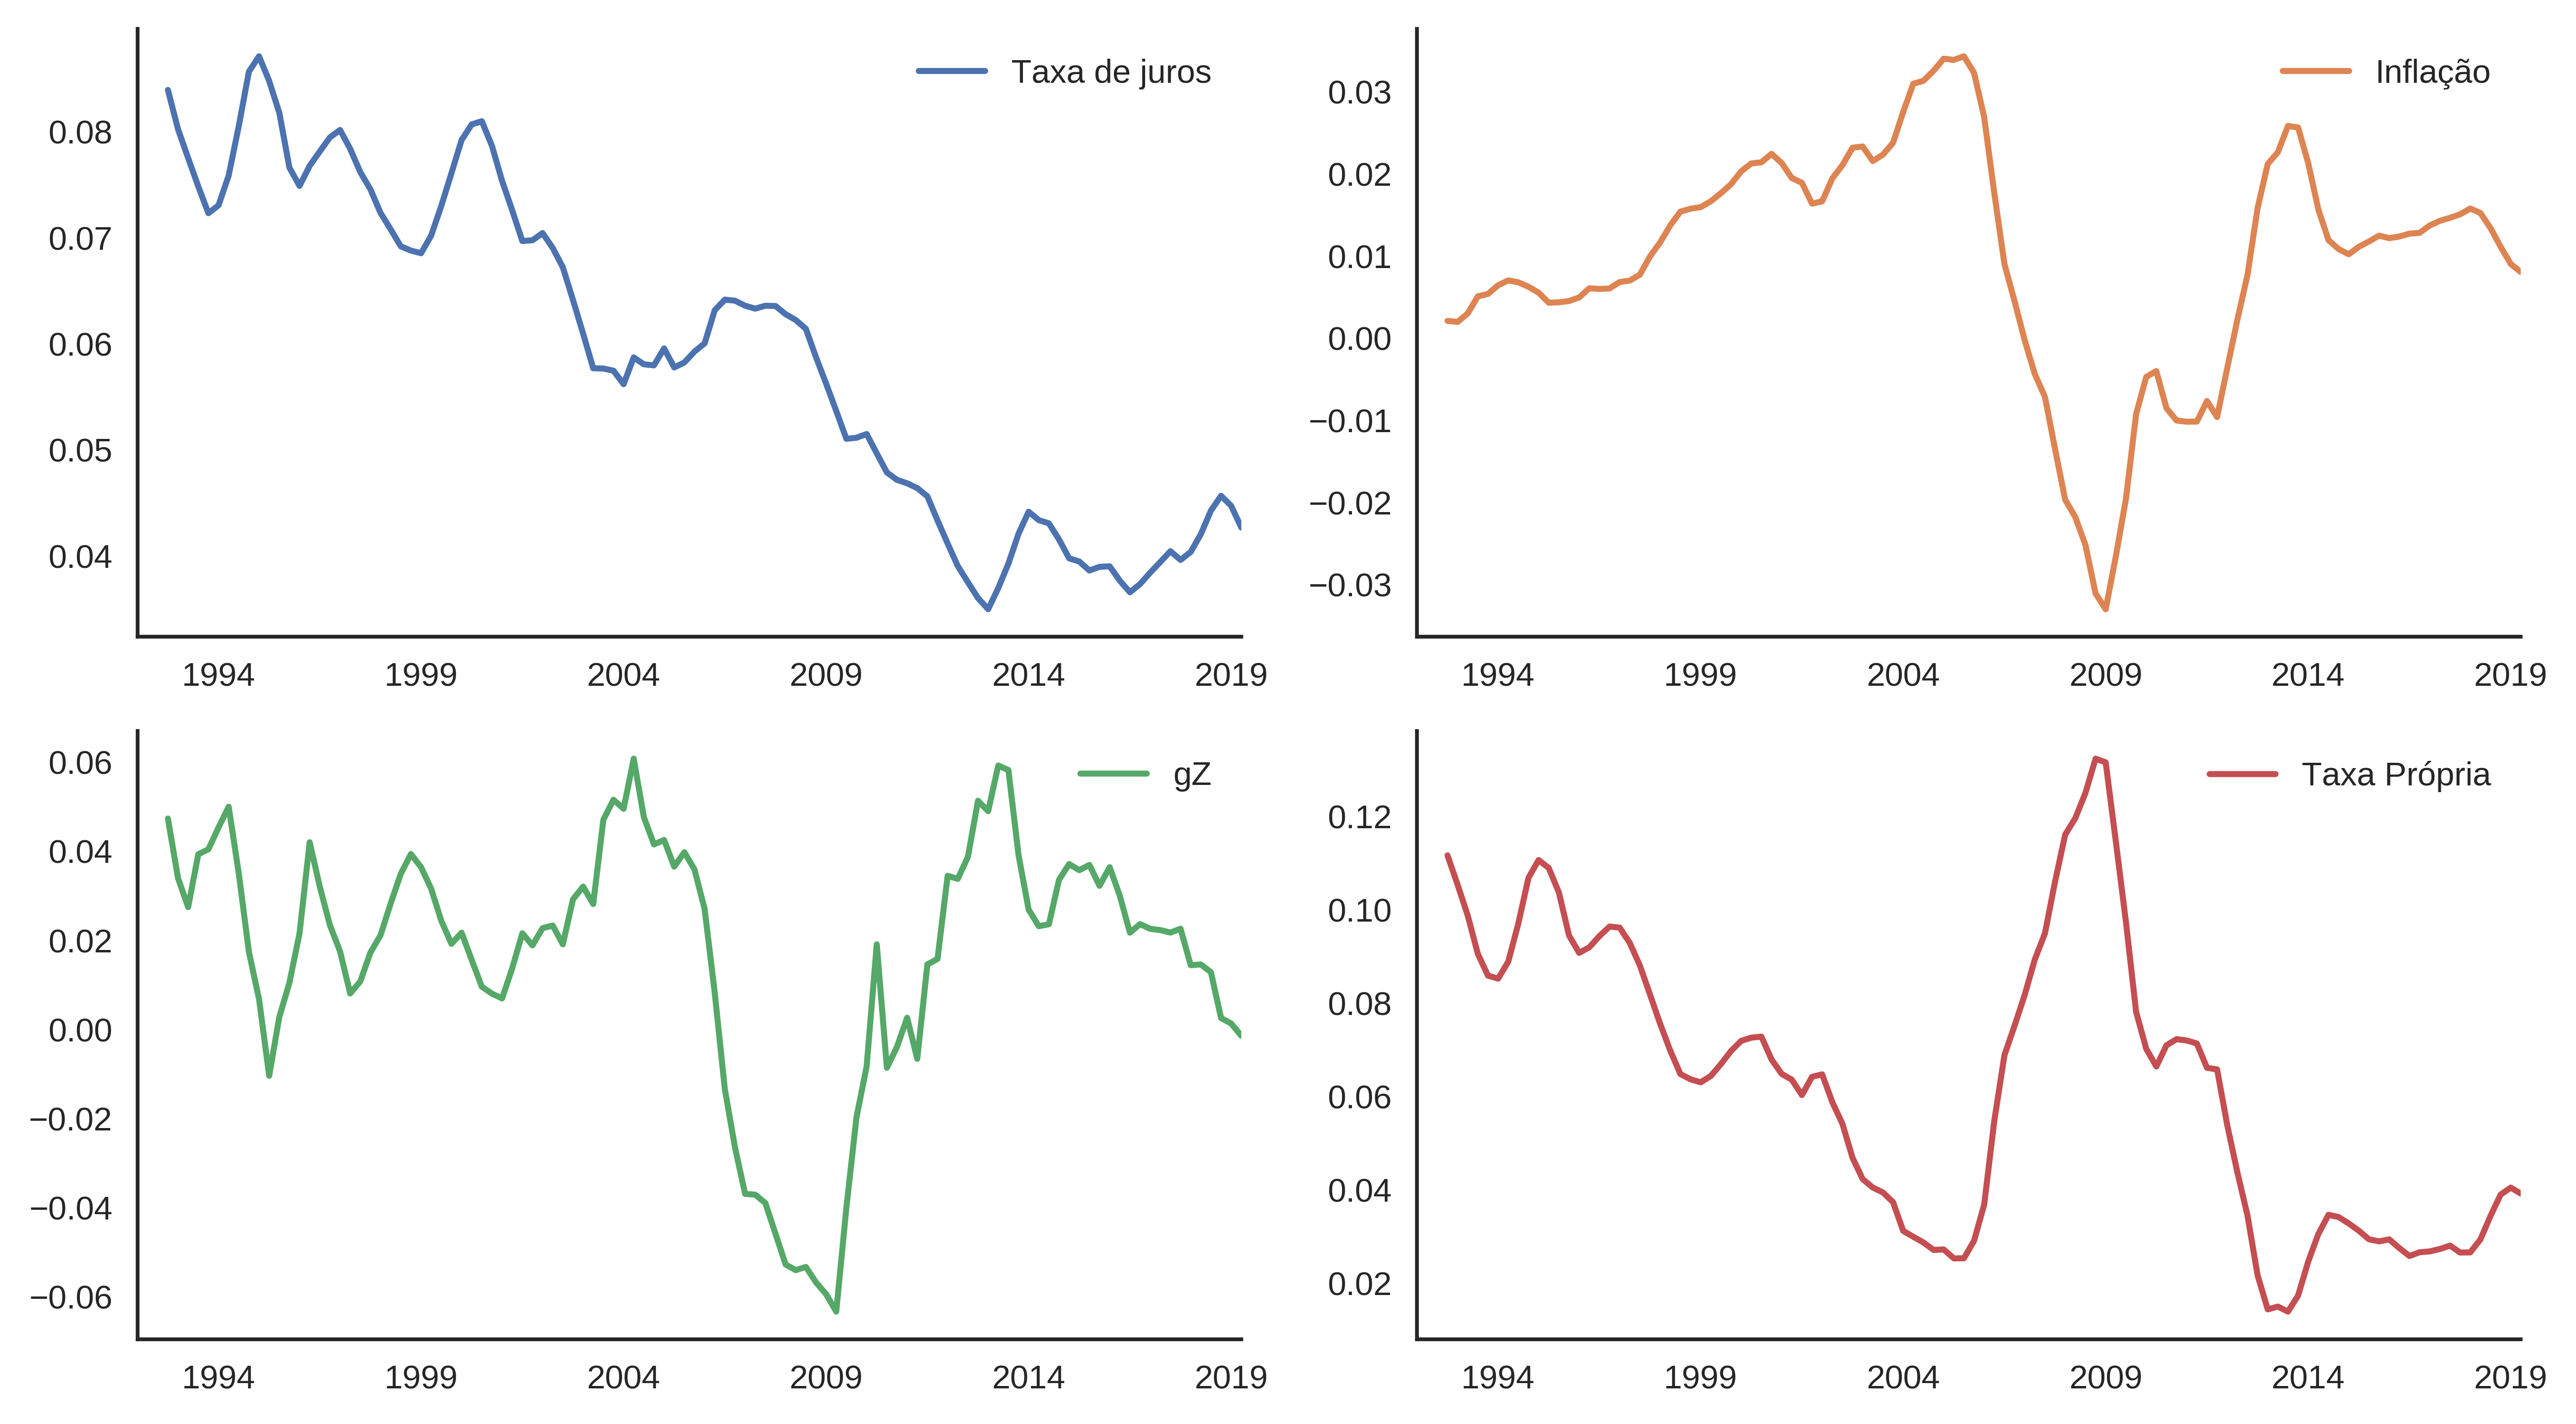
\includegraphics[width=\textwidth]{../../Dados/Fatos_Estilizados/figs/YeoJohnson_All.png}
	\caption*{\textbf{Fonte:} U.S. Bureau of Economic Analysis, elaboração própria}
\end{figure}


Dito isso, resta determinar a defasagem utilizada. Pelos critérios de informação, tanto o primeiro (trimestre) quanto o quarto \textit{lag} são elegíveis (ver tabela \ref{criterios}). Apesar de parcimonioso, a escolha da primeira defasagem não possui respaldo empírico. Se considerar o tempo médio de construção de imóveis desde a aprovação até a conclusão, verifica-se que deve-se incluir \textit{ao menos} o segundo \textit{lag} para incorporar as residências construídas pela motivação de obter ganhos de capital na revenda que só se realizada uma vez concluída a construção (ver figura \ref{meses}). Tal procedimento, no entanto, não é suficiente para determinar a seleção do \textit{lag} a ser utilizado. Dado que o fluxo de novos imóveis é significativamente inferior ao estoque existente, o efeito da variação dos preços se verifica mesmo com as construções não concluídas, ou seja, decorre das expectativas em relação à inflação futura.  Tal elemento seria captado pela taxa própria \textit{esperada}. No entanto, não há uma série para tal de modo que as defasagens são uma primeira aproximação para a taxa esperada.


\begin{table}[htb]
	\caption{Seleção da ordem do VECM (* indica o mínimo)}
	\label{criterios}
\begin{center}
\begin{tabular}{lcccc}
\toprule
            & \textbf{AIC} & \textbf{BIC} & \textbf{FPE} & \textbf{HQIC}  \\
\midrule
\textbf{0}  &      -14.96  &     -14.69*  &   3.186e-07  &      -14.85*   \\
\textbf{1}  &      -14.99  &      -14.61  &   3.100e-07  &       -14.83   \\
\textbf{2}  &      -14.96  &      -14.47  &   3.196e-07  &       -14.76   \\
\textbf{3}  &      -14.98  &      -14.39  &   3.112e-07  &       -14.74   \\
\textbf{4}  &      -15.09  &      -14.39  &   2.806e-07  &       -14.81   \\
\textbf{5}  &      -15.09  &      -14.28  &   2.802e-07  &       -14.77   \\
\textbf{6}  &     -15.12*  &      -14.20  &  2.735e-07*  &       -14.75   \\
\textbf{7}  &      -15.09  &      -14.06  &   2.840e-07  &       -14.67   \\
\textbf{8}  &      -15.05  &      -13.92  &   2.948e-07  &       -14.59   \\
\textbf{9}  &      -14.98  &      -13.73  &   3.188e-07  &       -14.48   \\
\textbf{10} &      -14.97  &      -13.62  &   3.238e-07  &       -14.42   \\
\textbf{11} &      -14.94  &      -13.48  &   3.358e-07  &       -14.35   \\
\textbf{12} &      -14.88  &      -13.31  &   3.603e-07  &       -14.24   \\
\textbf{13} &      -14.91  &      -13.24  &   3.511e-07  &       -14.24   \\
\textbf{14} &      -14.86  &      -13.07  &   3.763e-07  &       -14.13   \\
\textbf{15} &      -14.82  &      -12.93  &   3.934e-07  &       -14.06   \\
\bottomrule
\end{tabular}
%\caption{VECM Order Selection (* highlights the minimums)}
\end{center}
\caption*{\textbf{Fonte:} Elaboração própria}
\end{table}


\begin{figure}[H]
	\centering
	\caption{Tempo médio de construção (aprovação a conclusão) de imóveis para uma unidade familiar por propósito de construção exceto casas pré-fabricadas (1976-2018)}
	\label{meses}
	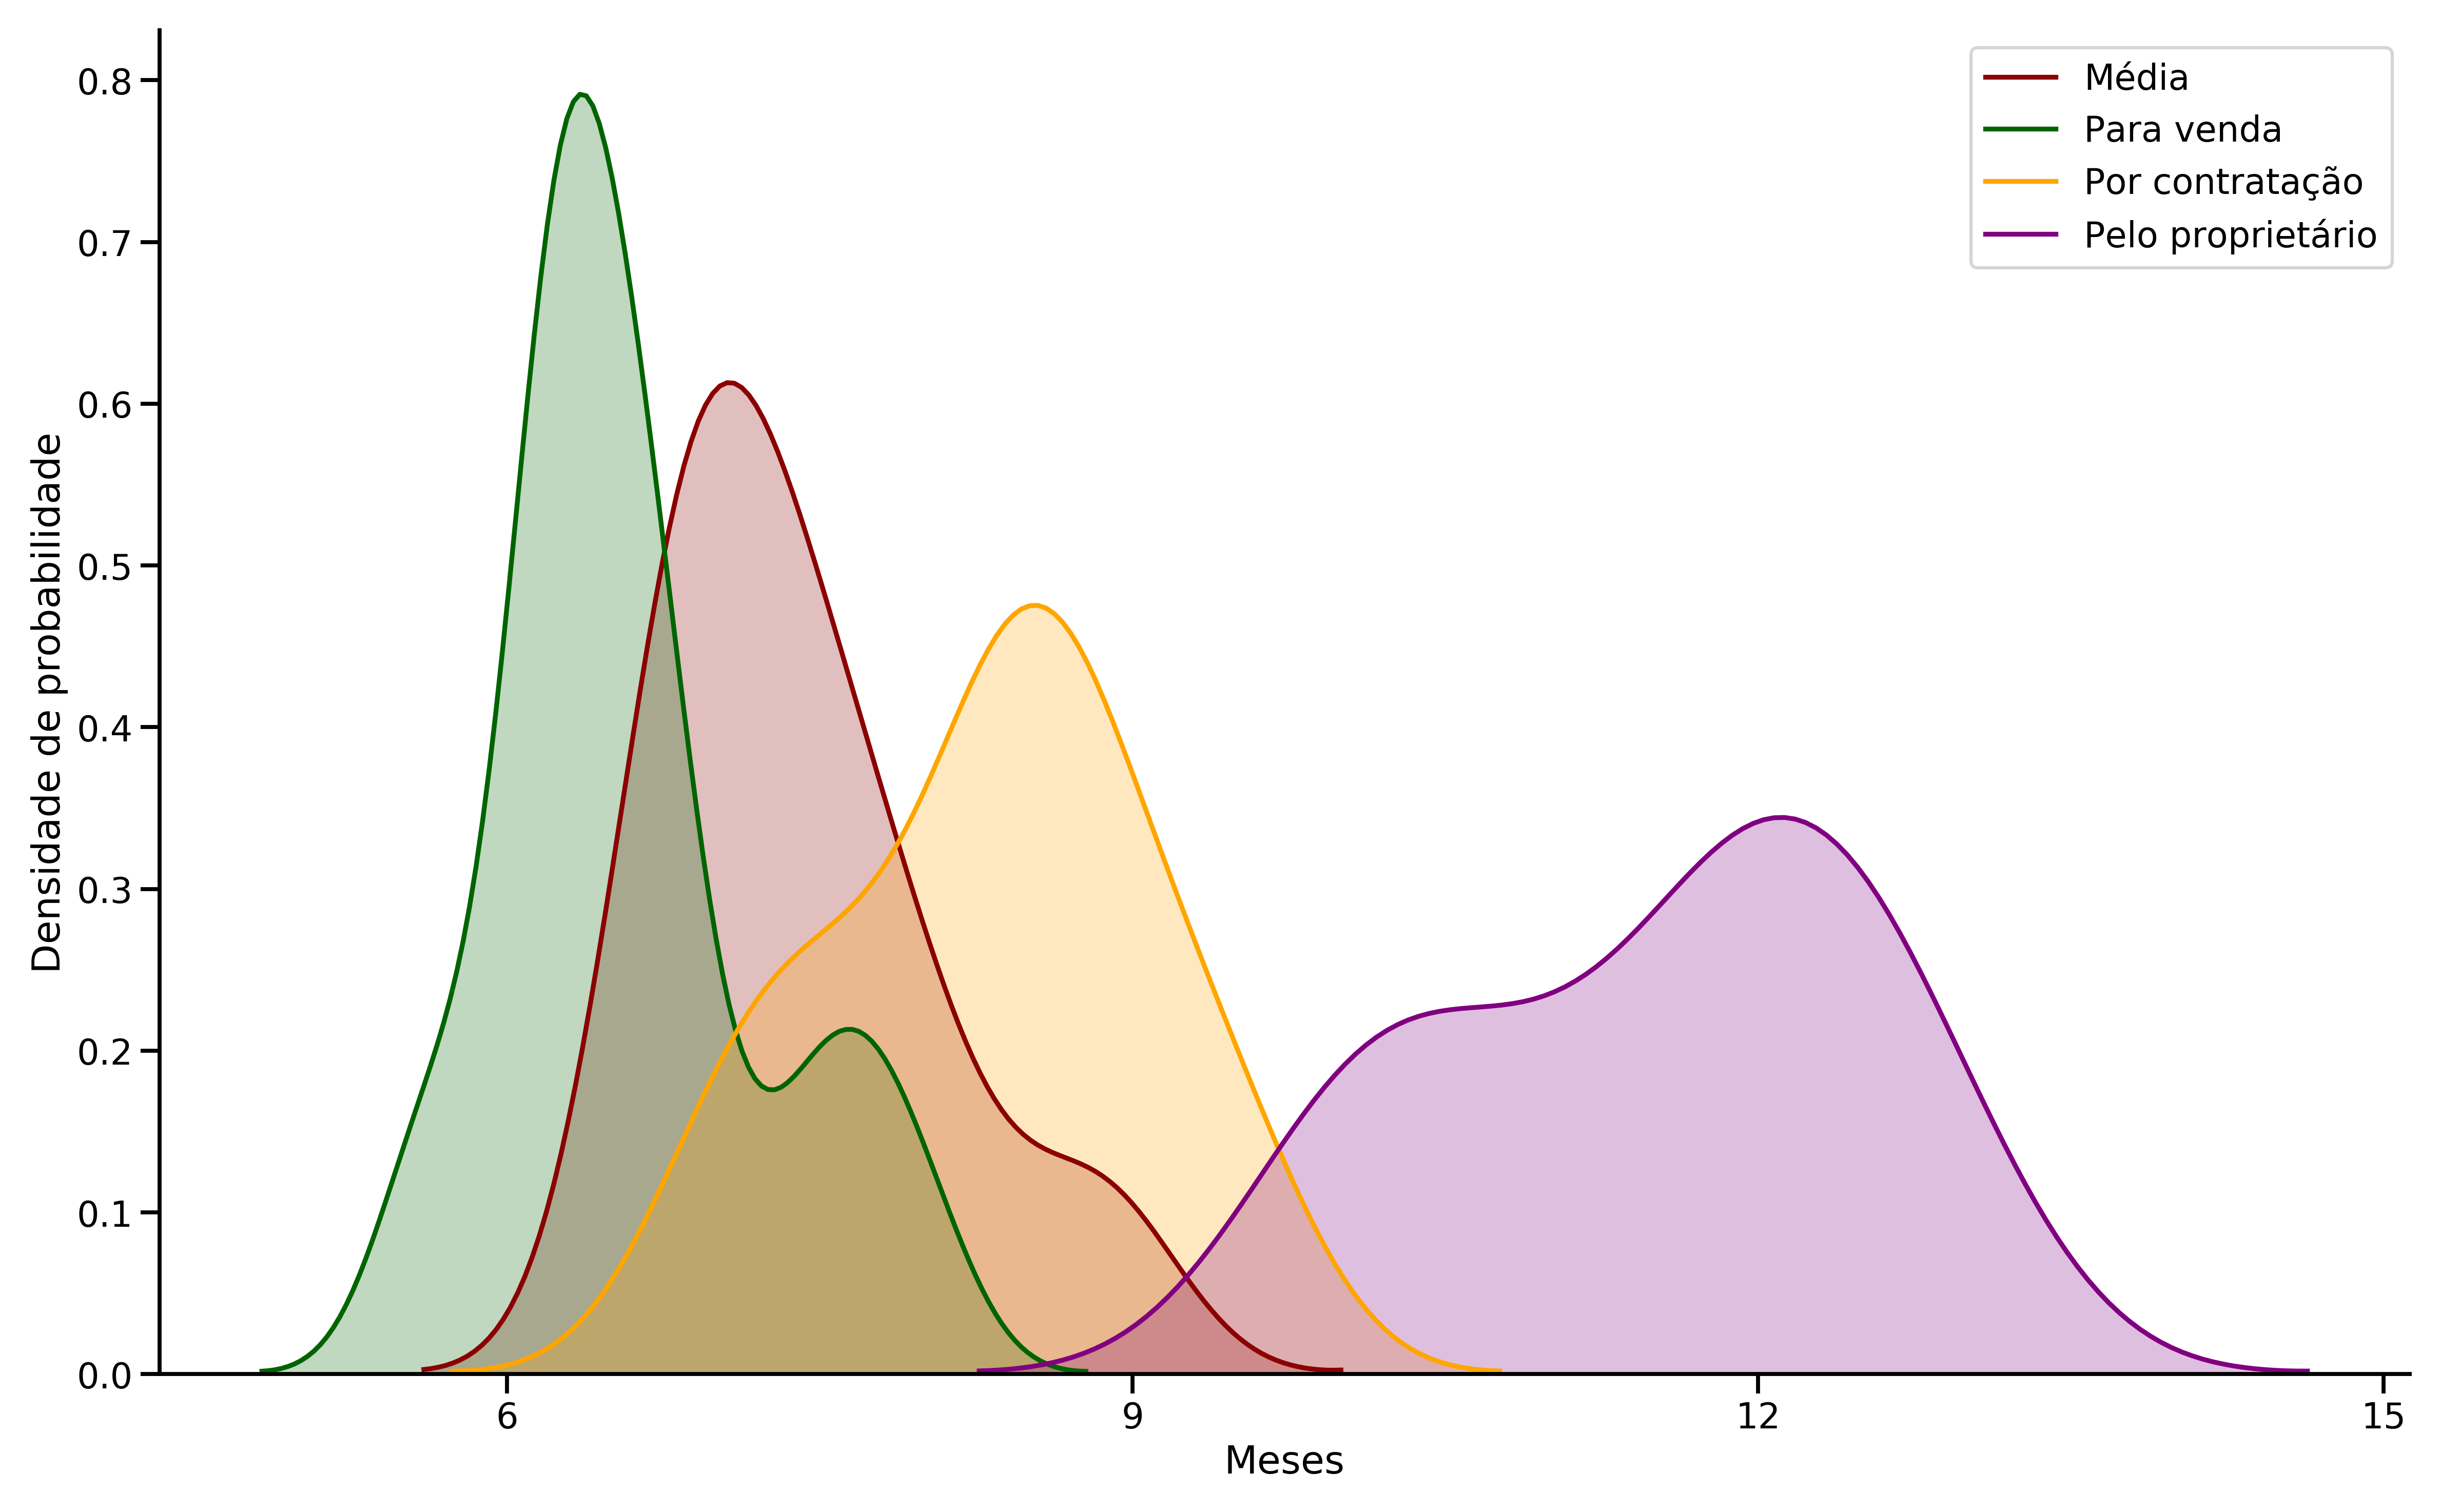
\includegraphics[width=\textwidth]{Fatos_Estilizados/Figs/Meses_contrucao.png}
	\caption*{\textbf{Fonte:} Survey of Construction (SOC), elaboração própria}
\end{figure}

Desse modo, uma alternativa é por meio de uma ``teoria prática do futuro'' --- como em \textcite[p.~214]{keynes_general_1937} --- em que o processo decisório para comprar um novo imóvel depende de componentes expectacionais/convenções associadas às observações passadas.
Em outras palavras, diante da inexistência de uma série para taxa própria esperada, será utilizada a defasagem desta variável como \textit{proxy}.
%TODO: Grifar
De forma a ilustrar tal relação, o gráfico \ref{defasagens} apresenta as variáveis de interesse frente aos \textit{lags} que minimizam os critérios de informação (respectivamente 1 e 4). 
Esse procedimento permite visualizar se existe alguma relação entre a taxa própria esperada (taxa efetiva defasada) e taxa de crescimento do investimento residencial\footnote{De modo a dar conta de não-linearidades, é apresentada a regressão quadrática entre ambas as variáveis (e o mesmo foi realizado para o gráfico inverso).}. Já a relação inversa, qual seja, da taxa de crescimento para a taxa própria não se verifica uma vez que, como visto, o fluxo de novos imóveis é bastante inferior o estoque de imóveis existente e, portanto, é esperado que tal relação não esteja presente. Em outras palavras, a especulação com o \textit{estoque}  de imóveis gera inflação desses ativos que, por conseguinte, afeta a construção de novos imóveis (\textit{fluxo}) e não o inverso\footnote{
	Cabe aqui destacar um aspecto particular da formação de preços dos imóveis: escassez de terra. Como consequência, a especulação com residências é, no limite, especulação com a terra (único recurso escasso envolvido em sua produção) e, portanto, é importante para a especulação com o estoque de imóveis. Ao discutir a formação de preços no mercado imobiliário, \textcite[p.~349, grifos adicionados]{leamer_housing_2007} pontua:
	
	\begin{citacao}
	\textit{It’s not the structure that has a volatile price; \textbf{it's the land}. Where there is plenty of buildable land, the response to an increase in demand for homes is mostly to build more, not to increase prices. Where there is little buildable land, the response to an increase in demand for homes is mostly a price increase, sufficient to discourage buyers enough to reequilibrate the supply and demand.}
	\end{citacao}	
}. 
%TODO Referência de terra ser escassa.
Essa inspeção, portanto, ilustra de forma bastante grosseira tal componente expectacional por meio da menor dispersão entre os pontos no gráfico inferior direito\footnote{Raciocínio semelhante pode ser encontrado em \textcite{girardi_autonomous_2015}}.  


\begin{figure}[htb]
	\centering
	\caption{Dispersão entre taxa própria e crescimento do investimento residencial: defasagens selecionadas a partir dos critérios de informação}
	\label{defasagens}
	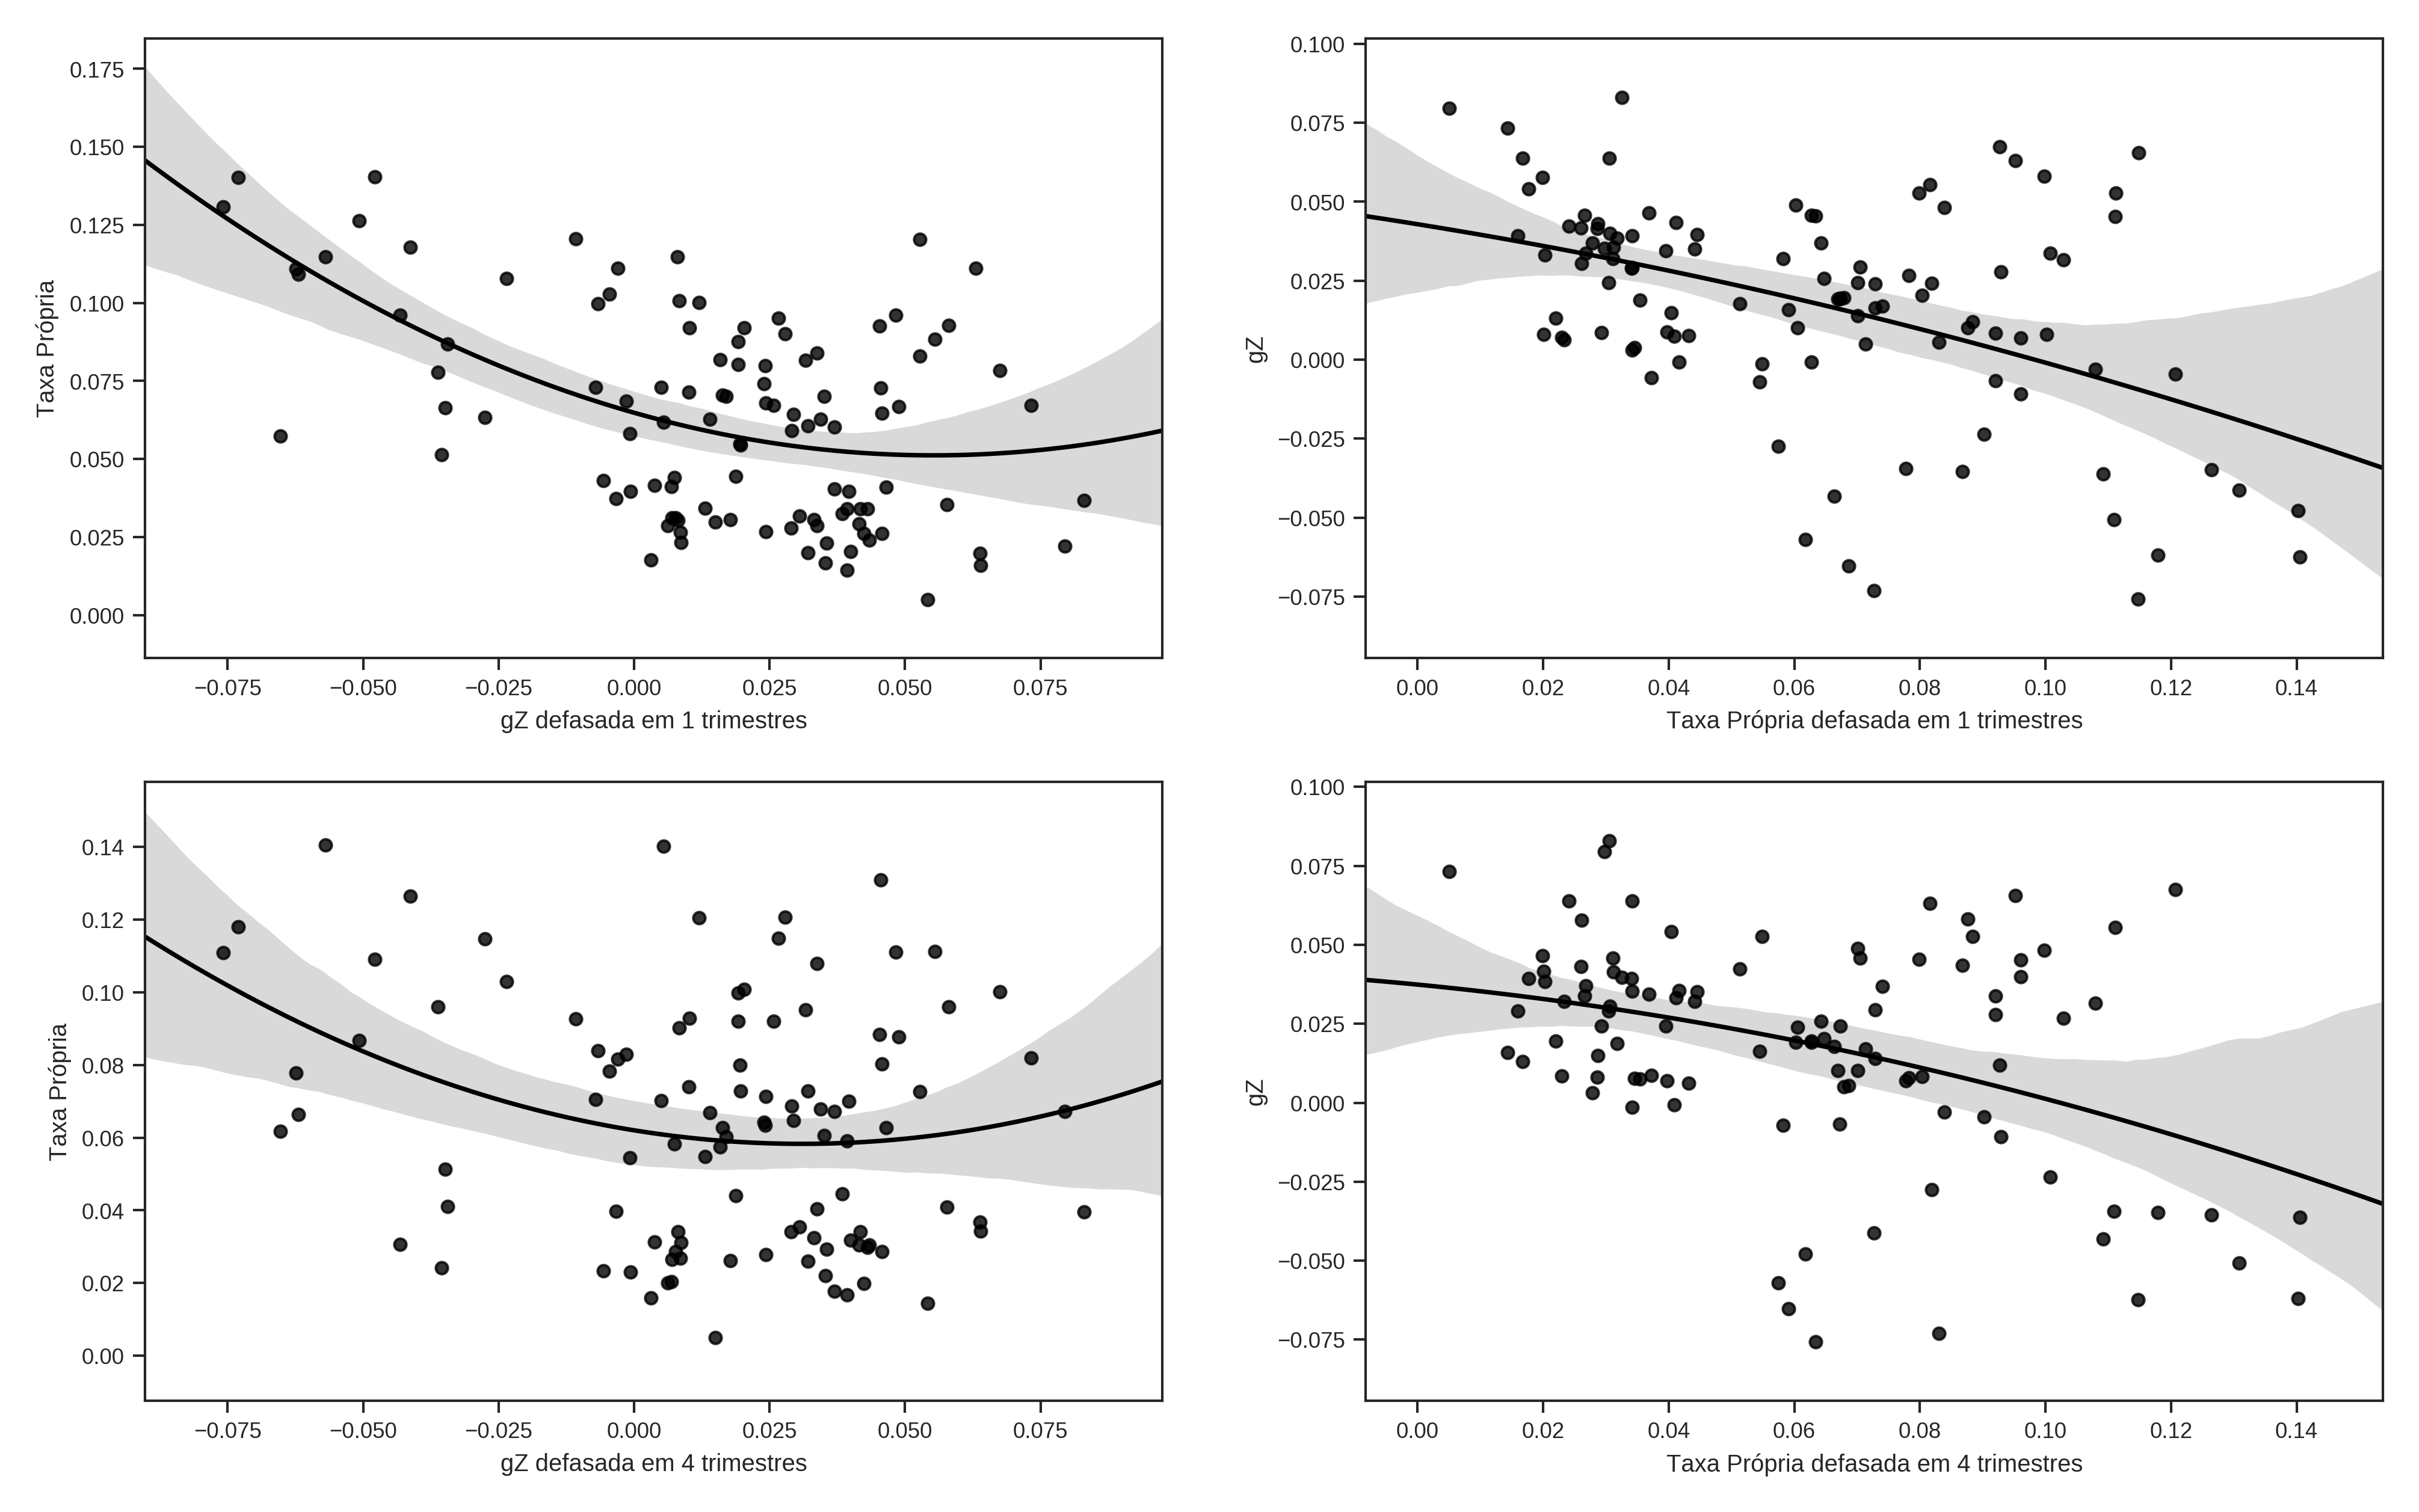
\includegraphics[width=\textwidth]{../../Modelo/SeriesTemporais/figs/VEC_Defasagens.png}
	\caption*{\textbf{Fonte:} Elaboração própria}
\end{figure}
%TODO Adicionar gráficos com defasagem 2


%TODO Modificar tabela da estimação

Uma vez selecionado o \textit{lag} que minimiza os critérios de informação e feita esta contextualização teórica da escolha das defasagens,  estima-se um VECM de ordem 4\footnote{Nota-se que tal defasagem, além de ser teoricamente justificada, também gera resíduos não heterocedásticos e sem correlação serial (ver tabela \ref{testes_resduos}).} cujos resíduos são apresentados no gráfico \ref{residuos} e resultados são expostos na tabela \ref{Estimacao}.
Começando pela relação de cointegração, verifica-se que é estatisticamente significante para ambas as equações de modo que as variáveis partilham uma relação (negativa) de longo prazo, ou seja, são cointegradas (fundamentando os pontos 1 e 4 da tabela \ref{resultados_esperados}).
Desse modo, a proposição de \textcite{teixeira_crescimento_2015} é corroborada por meio do coeficiente $\phi_1> 0$ e estatisticamente significante.
Além disso, os coeficientes $\gamma_{2,is}$ estimados são negativos seguindo os resultados esperados (6) do mesmo modo que a demanda por imóveis por motivos não-especulativos ($\phi_0$) é estatisticamente significante (resultado 5).
Adotando um nível de significância de 5\%, verifica-se que o parâmetro de correção de erro é estatisticamente significante apenas para a equação da taxa de crescimento do investimento residencial. Portanto, a variável $own$ é exogenamente fraca em relação a $g_{I_h}$ enquanto taxa própria Granger-causa $g_{I_h}$, validando os resultado esperados (2) e (3).
Já as relações de curto prazo entre taxa própria e $g_{I_h}$ (capturadas por $\beta_{1,is}$) não são estatisticamente significantes a 5\% \footnote{O resultado esperado (7) também pode ser confirmado a partir da inspeção da tabela \ref{Estimacao} em que apenas a quarta defasagem da taxa própria é estatisticamente significante nesta equação.}. Portanto, os resultados obtidos estão em linha com os esperados e podem ser resumidos nos seguintes termos: taxa própria de juros dos imóveis determina a --- mas não é determinada pela --- taxa de crescimento do investimento residencial e estas variáveis apresentam uma relação negativa de longo prazo.

\begin{table}[H]
	\centering
	\caption{Parâmetros da estimação (VECM)}
	\label{Estimacao}
\begin{threeparttable}
	\begin{tabular}{lcccccc}
		\hline \hline
		\textbf{Equação:} $own$ & \textbf{coef} & \textbf{std err} & \textbf{z} & \textbf{P$> |$z$|$} & \textbf{[0.025} & \textbf{0.975]}  \\
		\midrule
		\textbf{$\delta_{1}$}      &   -1.632e-05  &      4.4e-05     &    -0.371  &         0.710        &       -0.000    &     6.98e-05     \\
		\textbf{$\gamma_{1,1}$ ($L_1$ $own$)} &       0.0381  &        0.111     &     0.342  &         0.732        &       -0.180    &        0.256     \\
		\textbf{$\beta_{1,1}$ ($L_1 g_{I_h}$)}           &       0.0738  &        0.083     &     0.887  &         0.375        &       -0.089    &        0.237     \\
		\textbf{$\gamma_{1,2}$ ($L_2$ $own$)} &      -0.0032  &        0.110     &    -0.029  &         0.977        &       -0.218    &        0.212     \\
		\textbf{$\beta_{1,2}$ ($L_2 g_{I_h}$)}           &       0.1115  &        0.082     &     1.366  &         0.172        &       -0.048    &        0.272     \\
		\textbf{$\gamma_{1,3}$ ($L_3$ $own$)} &       0.0757  &        0.118     &     0.642  &         0.521        &       -0.156    &        0.307     \\
		\textbf{$\beta_{1,3}$ ($L_3 g_{I_h}$)}           &       0.1080  &        0.069     &     1.563  &         0.118        &       -0.027    &        0.243     \\
		\textbf{$\gamma_{1,4}$ ($L_4$ $own$)} &       0.2649  &        0.119     &     2.230  &         0.026$^{***}$        &        0.032    &        0.498     \\
		\textbf{$\beta_{1,4}$ ($L_4 g_{I_h}$)}           &      0.0583  &        0.054     &    1.089  &         0.276        &       -0.047    &       0.163     \\
		\midrule
		\textbf{Equação:} $g_{I_h}$ & \textbf{coef} & \textbf{std err} & \textbf{z} & \textbf{P$> |$z$|$} & \textbf{[0.025} & \textbf{0.975]}  \\
		\midrule
		\textbf{$\delta_{2}$}      &      -0.0003  &     6.96e-05     &    -3.848  &         0.000$^{***}$        &       -0.000    &       -0.000     \\
		\textbf{$\gamma_{2,1}$ ($L_1$ $own$)} &      -0.1747  &        0.176     &    -0.991  &         0.322        &       -0.520    &        0.171     \\
		\textbf{$\beta_{2,1}$ ($L_2 g_{I_h}$)}           &      -0.4203  &        0.132     &    -3.191  &         0.001$^{***}$        &       -0.678    &       -0.162     \\
		\textbf{$\gamma_{2,2}$ ($L_2$ $own$)} &      -0.9997  &        0.174     &    -5.752  &         0.000$^{***}$        &       -1.340    &       -0.659     \\
		\textbf{$\beta_{2,2}$ ($L_1 g_{I_h}$)}           &      -0.4596  &        0.129     &    -3.555  &         0.000$^{***}$        &       -0.713    &       -0.206     \\
		\textbf{$\gamma_{2,3}$ ($L_3$ $own$)} &      -0.5863  &        0.187     &    -3.137  &         0.002$^{***}$        &       -0.953    &       -0.220     \\
		\textbf{$\beta_{2,3}$ ($L_3 g_{I_h}$)}           &      -0.1991  &        0.109     &    -1.820  &         0.069*        &       -0.414    &        0.015     \\
		\textbf{$\gamma_{2,4}$ ($L_4$ $own$)} &      -0.5350  &        0.188     &    -2.844  &         0.004$^{***}$        &       -0.904    &       -0.166     \\
		\textbf{$\beta_{2,4}$ ($L_4 g_{I_h}$)}           &      -0.2444  &        0.085     &    -2.885  &         0.004$^{***}$        &       -0.411    &       -0.078     \\
		\midrule
		\textbf{Correção de Erro} & \textbf{coef} & \textbf{std err} & \textbf{z} & \textbf{P$> |$z$|$} & \textbf{[0.025} & \textbf{0.975]}  \\
		\midrule
		\textbf{$\alpha_1$} &      -0.0232  &        0.071     &    -0.328  &         0.743        &       -0.162    &        0.116     \\
		\textbf{$\alpha_2$} &      -0.4245  &        0.112     &    -3.784  &         0.000$^{***}$        &       -0.644    &       -0.205     \\
		\midrule
		\textbf{Relação de Cointegração} & \textbf{coef} & \textbf{std err} & \textbf{z} & \textbf{P$> |$z$|$} & \textbf{[0.025} & \textbf{0.975]}  \\
		\midrule
		\textbf{$\phi_{1,1}$} &       1.0000  &            0     &         0  &         0.000$^{***}$        &        1.000    &        1.000     \\
		\textbf{$\phi_{1,2}$} &       1.2835  &        0.149     &     8.599  &         0.000$^{***}$        &        0.991    &        1.576     \\
		\textbf{$\phi_0$}  &      -0.1131  &        0.009     &   -12.528  &         0.000$^{**}$       &       -0.131    &       -0.095     \\
		\hline
		\hline
	\end{tabular}
	%\caption{Det. terms outside the coint. relation & lagged endog. parameters for equation $own$}
\footnotesize{(*) Estatisticamente significante a 10\%; (**) Estatisticamente significante a 5\%; (***) Estatisticamente significante a 1\%.}
\end{threeparttable}
	\caption*{\textbf{Fonte:} Elaboração própria}
\end{table}

\begin{figure}[H]
	\centering
	\caption{Inspeção dos resíduos da estimação}
	\label{residuos}
	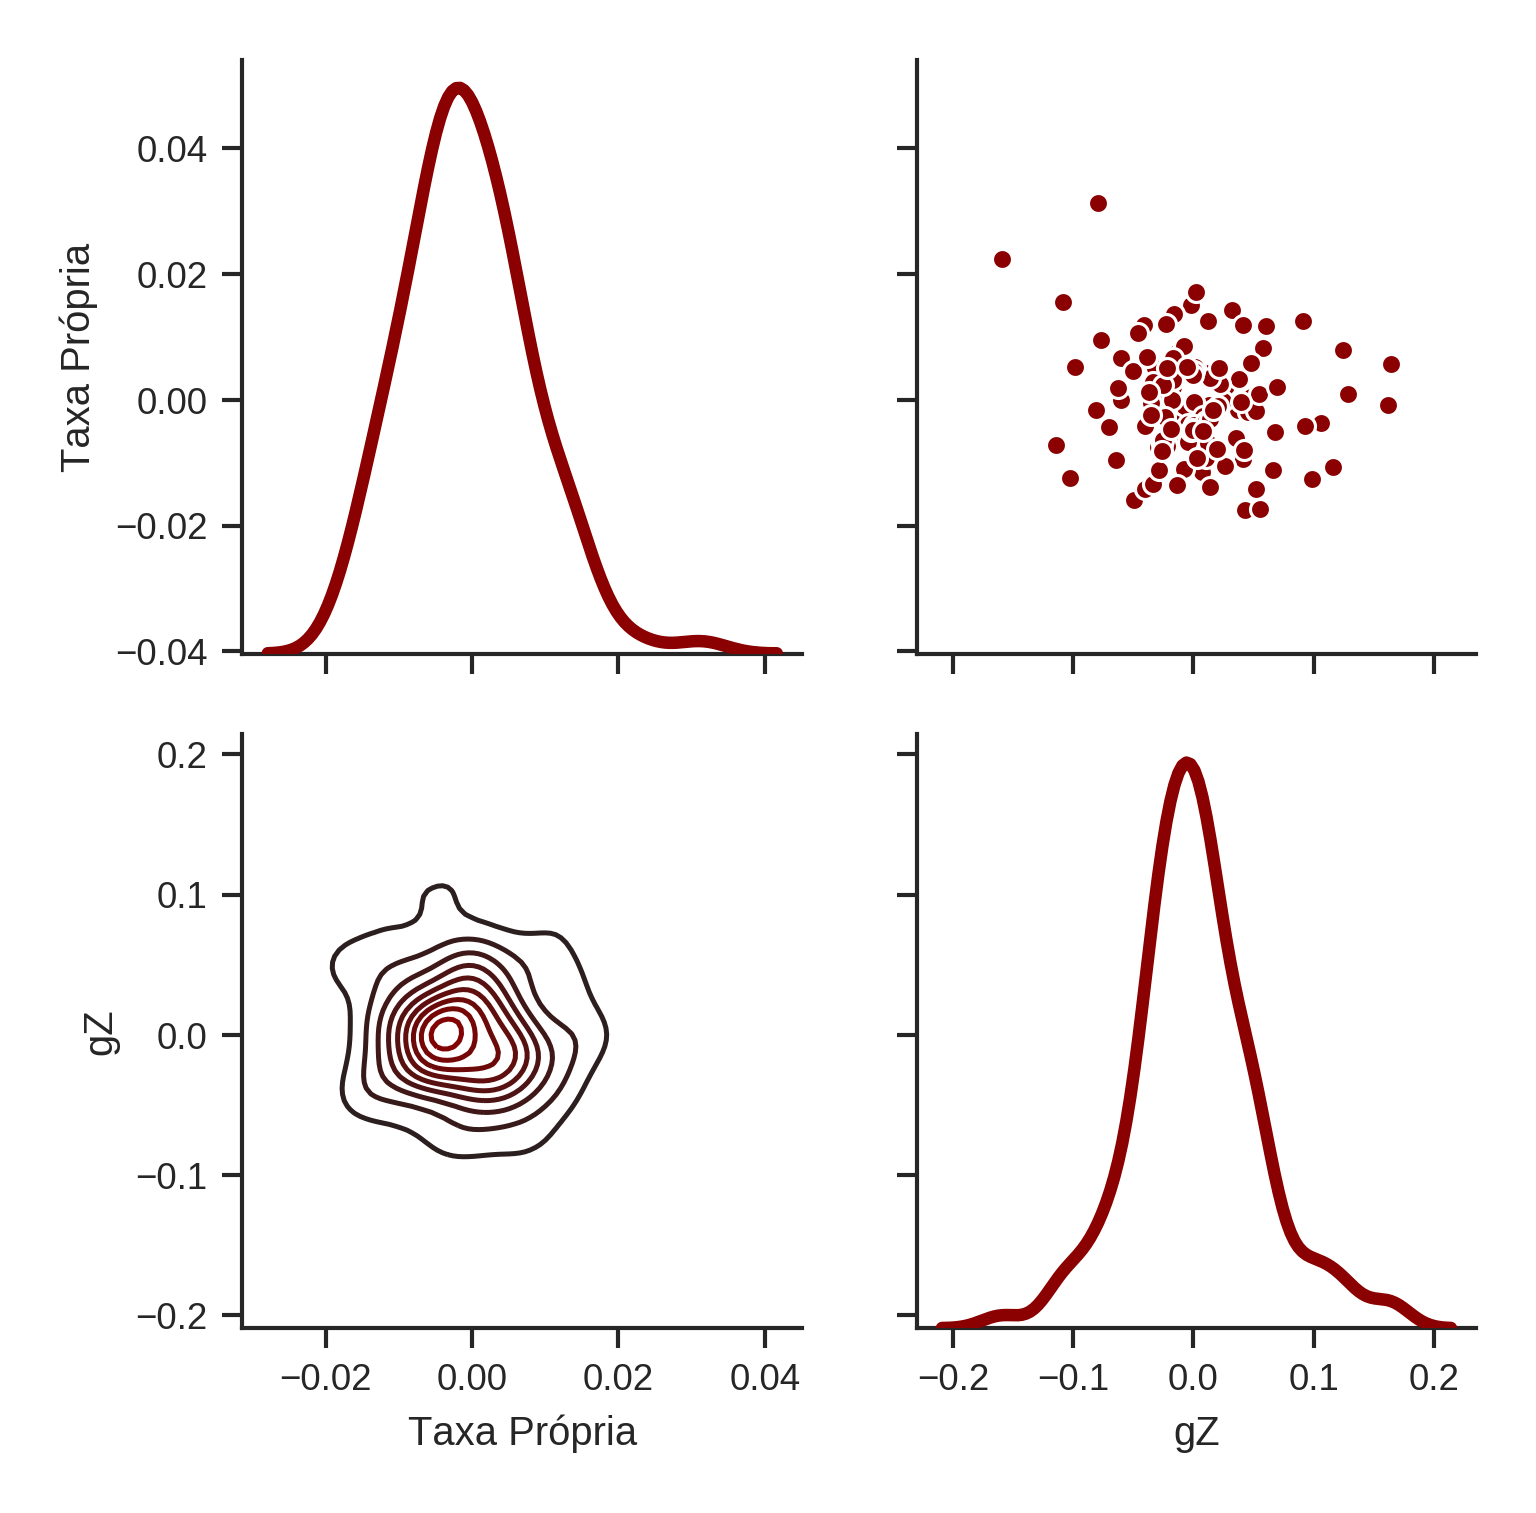
\includegraphics[height=.4\textheight]{../../Modelo/SeriesTemporais/figs/Residuos_4VECM.png}
	\caption*{\textbf{Fonte:} Elaboração própria}
\end{figure}


% Please add the following required packages to your document preamble:
% \usepackage{multirow}
% \usepackage{graphicx}
\begin{table}[H]
\centering
\caption{Testes de hipóteses sobre os resíduos}
\label{testes_resduos}
	\begin{threeparttable}
\begin{tabular}{l|c|c|c}
\hline
\multicolumn{2}{l|}{} & \textbf{Estatística} & \textbf{p-valor} \\ \hline
\textbf{Autocorrelação serial}\tnote{a} & Sistema & 54.51 & 0.093 \\ \hline
\multirow{2}{*}{\textbf{Homocedasticidade}\tnote{b}} & $own$ & 1.863 & 0.175 \\ \cline{2-4} 
 & $g_{I_h}$ & 3.080 & 0.082 \\ \hline
\textbf{Normalidade}\tnote{c} & Sistema & 46.64 & 0.000 \\ \hline
\end{tabular}%
\begin{tablenotes}\footnotesize
	\item [a] Teste de Portmanteau ajustado para até o 15º \textit{lag}. H0: autorocorrelação serial até o \textit{lag} selecionado é zero.
	\item [b] Teste ARCH-LM. H0: Resíduos são homocedásticos.
	\item [c] Teste de Jarque-Bera. H0: Resíduos provém de uma distribuição normal.
\end{tablenotes}
\end{threeparttable}
\caption*{\textbf{Fonte:} Elaboração própria}
\end{table}

Uma forma de verificar a capacidade explicativa da taxa própria para $g_{I_h}$ é por meio da decomposição da variância da previsão (FEVD) como no gráfico \ref{fevd}\footnote{Também é importante destacar que dado o número de variáveis (duas), a ordenação de Choleski é suficiente para analisar a função resposta ao impulso uma vez que gera uma matriz semelhante a de um VECM estrutural. 
}. Verifica-se que desde o primeiro trimestre a taxa própria contribui para $g_{I_h}$ enquanto o inverso não é válido. Adicionalmente, é notável que tal contribuição é crescente e maior que 50\% para além do 3º trimestre. Portanto, a taxa própria é explicada principalmente por ela mesma e explica $g_{I_h}$ consideravelmente.

\begin{figure}[htb]
	\centering
	\caption{Decomposição da variância da previsão}
	\label{fevd}
	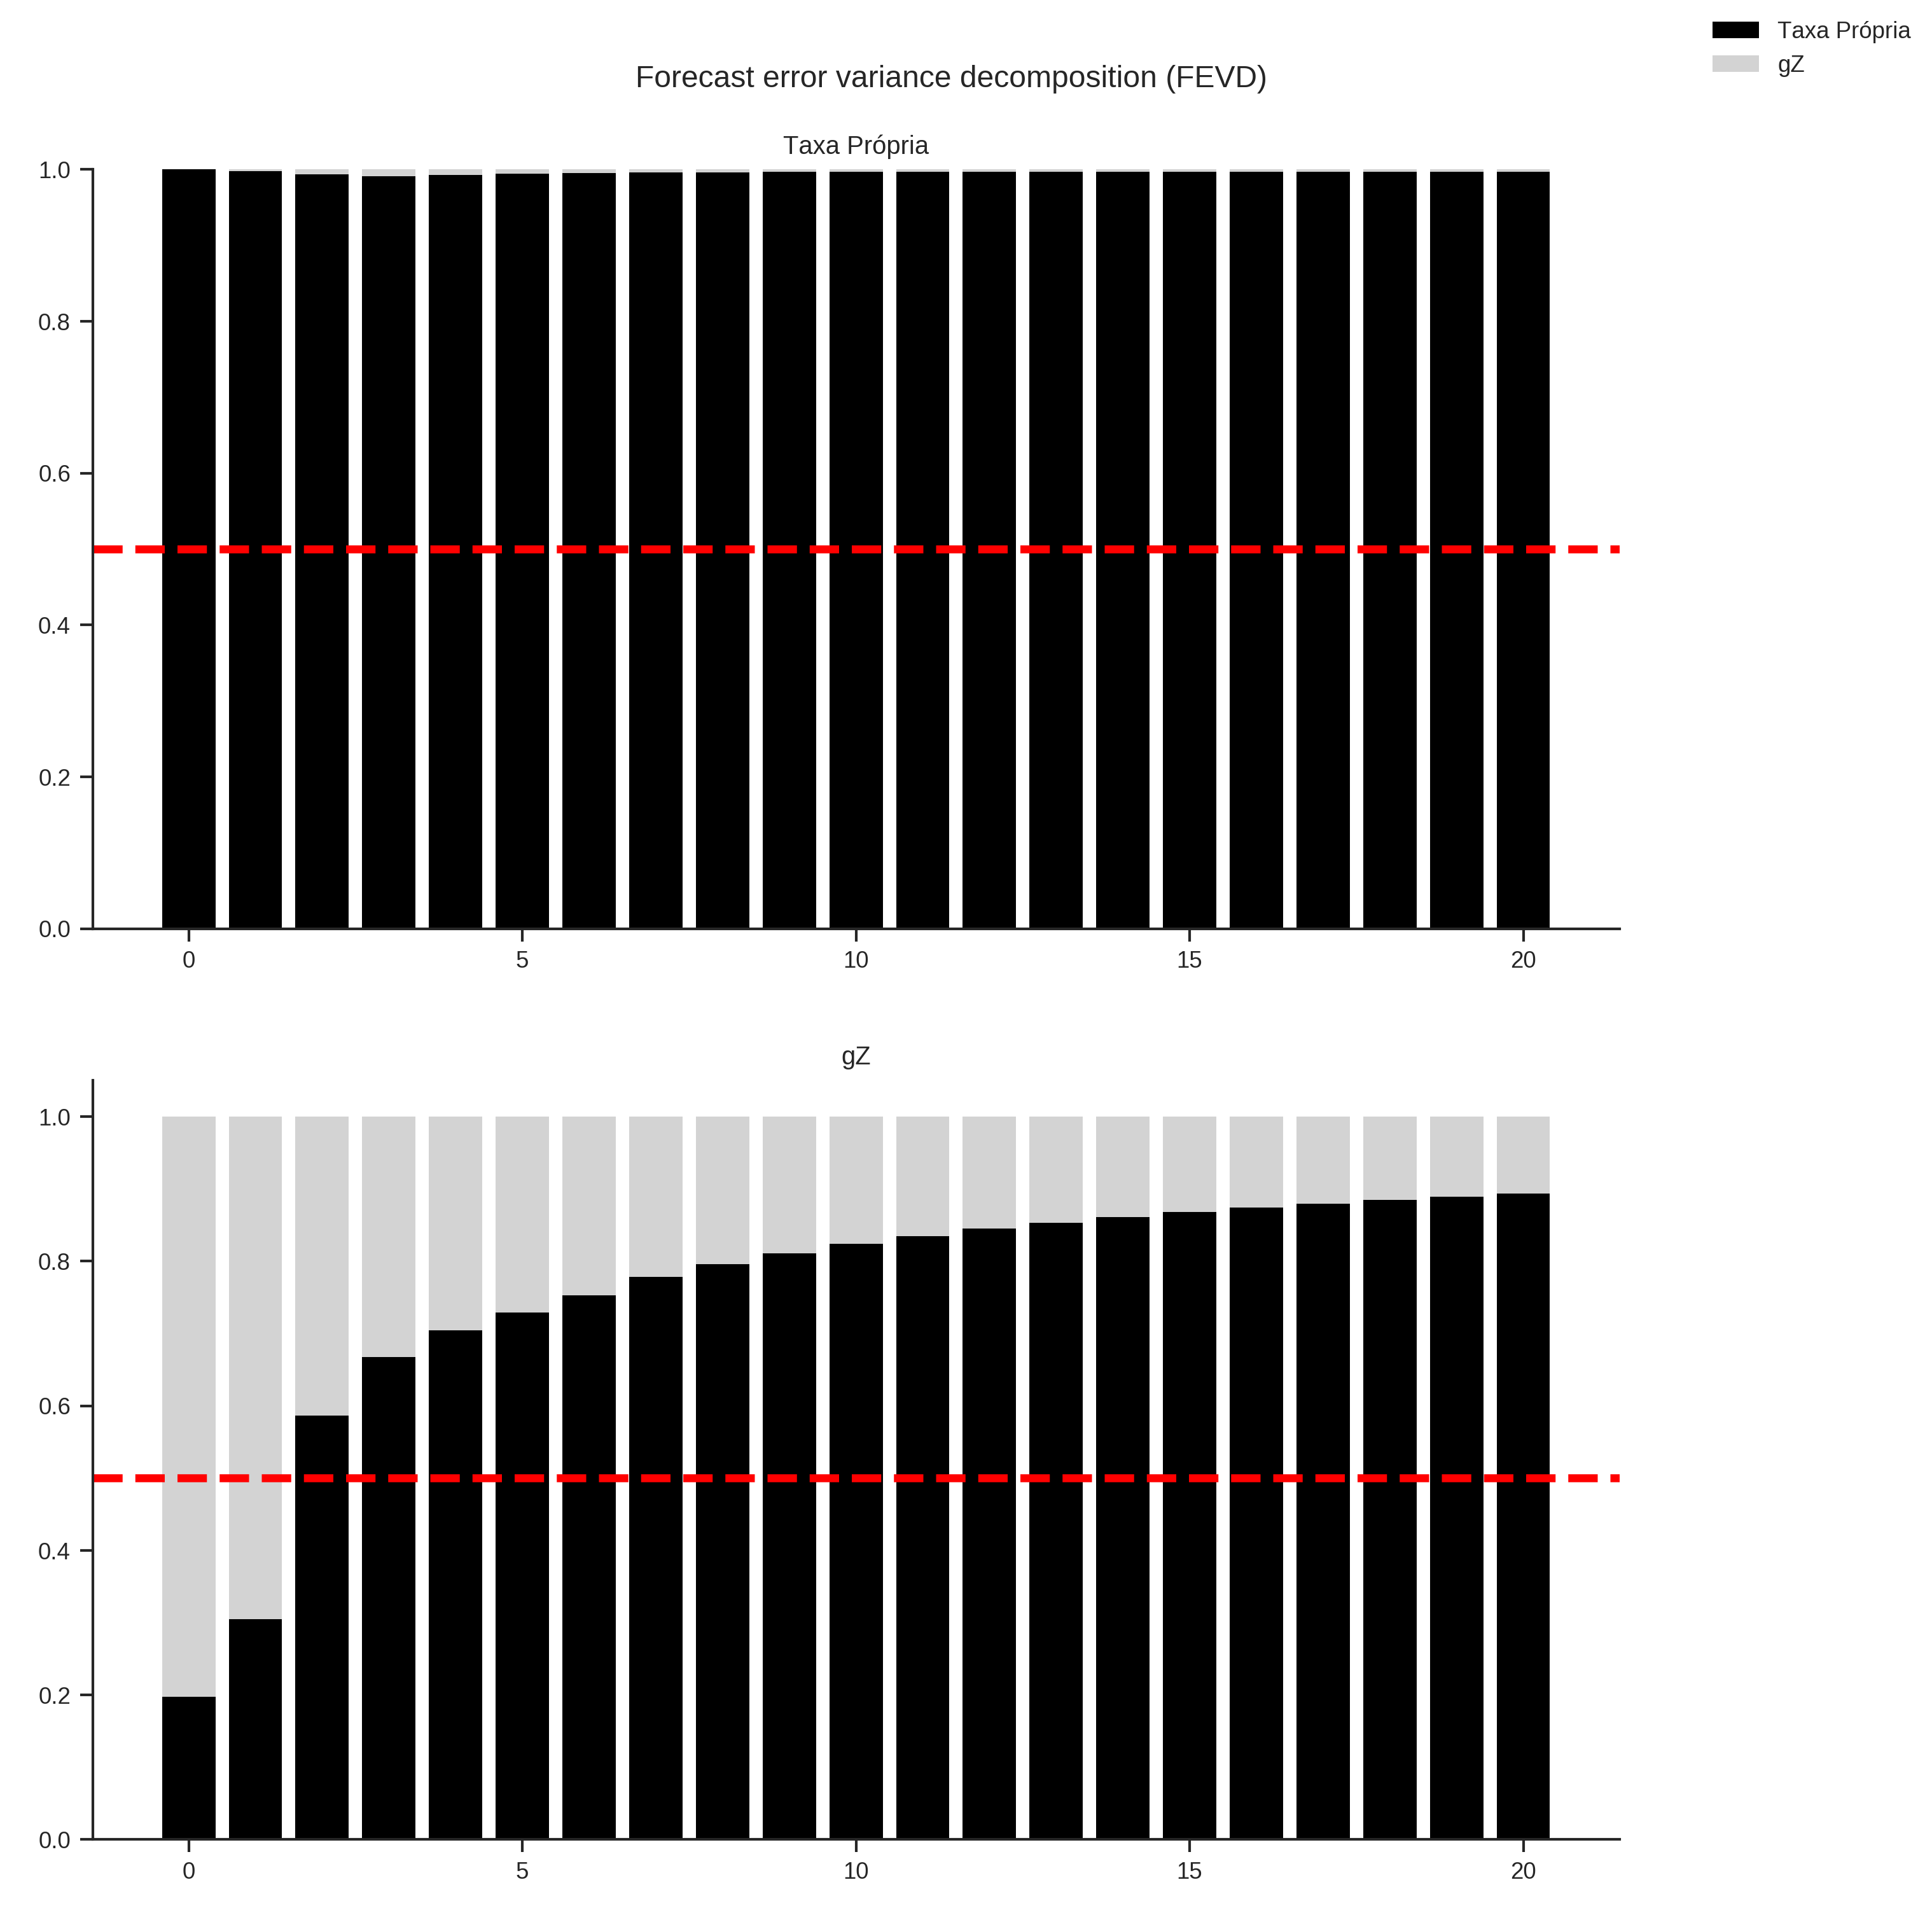
\includegraphics[width=\textwidth]{../../Modelo/SeriesTemporais/figs/FEVD_VECMpython_TxPropria.png}
	\caption*{\textbf{Fonte:} Elaboração própria}
\end{figure}


Adiante, é apresentado o gráfico da função impulso resposta ortogonalizada (gráfico \ref{irf}) --- grosso modo, as conclusões da FEVD se estendem também para os choques --- em que são avaliados os impactos no aumento de um desvio-padrão em uma das variáveis endógenas no primeiro período apenas.
%TODO Checar
A partir deste gráfico, verifica-se que o sistema é estável uma vez que os efeitos do aumento de $g_{I_h}$ sobre $g_{I_h}$ é amortecido ao longo do tempo enquanto os efeitos da taxa própria sobre a ela mesma são persistentes mas não explosivos.
Já os efeitos de $g_{I_h}$ sobre a taxa própria são nulos uma vez que o intervalo de confiança sempre abrange o zero. Por fim, e este é o resultado relevante, dados os objetivos, é o efeito negativo considerável e duradouro da taxa própria sobre $g_{I_h}$, confirmando a tese de \textcite{teixeira_crescimento_2015}.
Em resumo, as funções resposta ao impulso indicam que o aumento da taxa de juros das hipotecas (aumento na Taxa Própria) impacta negativamente na taxa de crescimento residencial enquanto o aumento da inflação de ativos implica no inverso. 
%alinhado com os resultados de \textcite{huang_is_2018} para o longo prazo.
%podendo estar associado aos gastos com aprimoramento residencial uma vez encerradas as construções (também contabilizado como investimento residencial).


\begin{figure}[H]
	\centering
	\caption{Função impulso resposta ortogonalizada}
	\label{irf}
	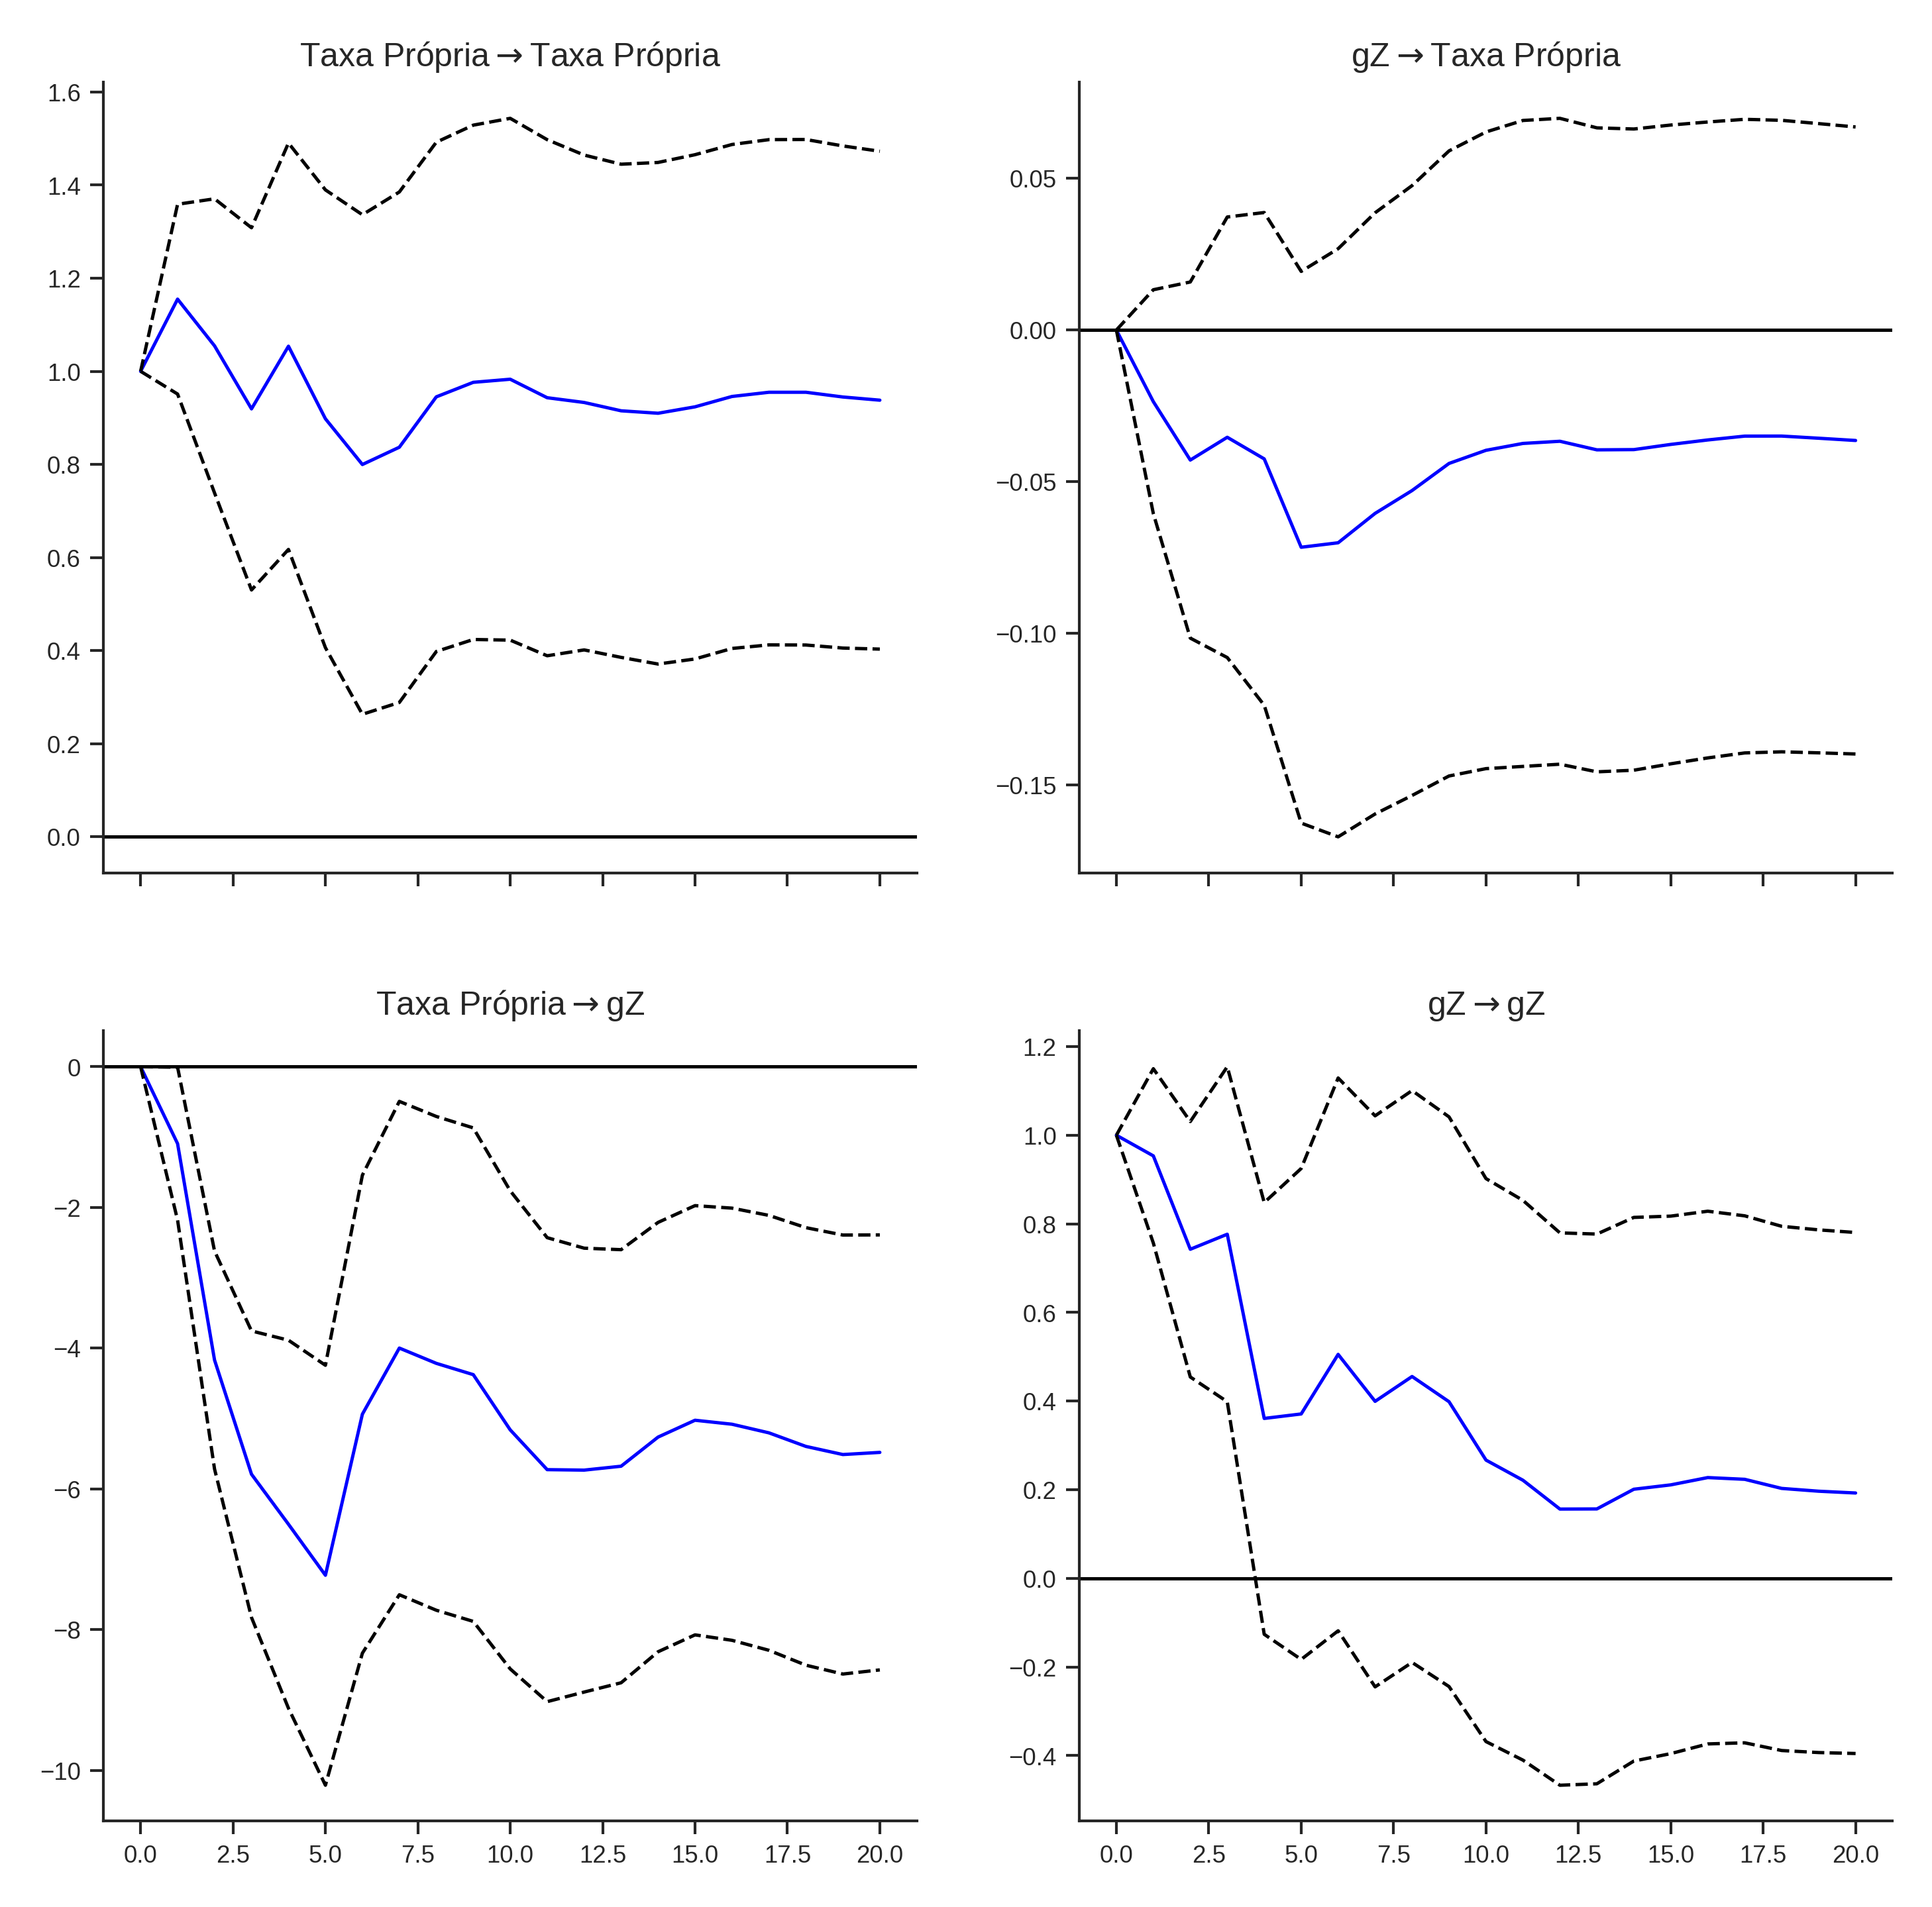
\includegraphics[width=\textwidth]{../../Modelo/SeriesTemporais/figs/Impulso_VECM.png}
	\caption*{\textbf{Fonte:} Elaboração própria}
\end{figure}

Dos resultados apresentados acima, verifica-se que a taxa própria de juros dos imóveis tem uma capacidade explicativa significativa. Vale destacar que apesar de amplitude das defasagens selecionadas, o modelo estimado é bastante parcimonioso em termos das variáveis utilizadas. Desse modo, considerando o grau de parcimônia e a robustez dos resultados, conclui-se que é um modelo satisfatório para explicar a taxa de crescimento do investimento residencial. 
%Diante da qualidade do ajuste, o gráfico \ref{previsao} apresenta a previsão do modelo 4 passos a frente. 
%Avaliando o últimos resultados disponíveis das contas nacionais e estimativas da taxa própria, verifica-se uma previsão satisfatória uma vez que tanto $g_{I_h}$ reduz quanto a taxa própria aumenta.

\begin{comment}
\begin{figure}[H]
	\centering
	\caption{Previsão 4 passos a frente}
	\label{previsao}
	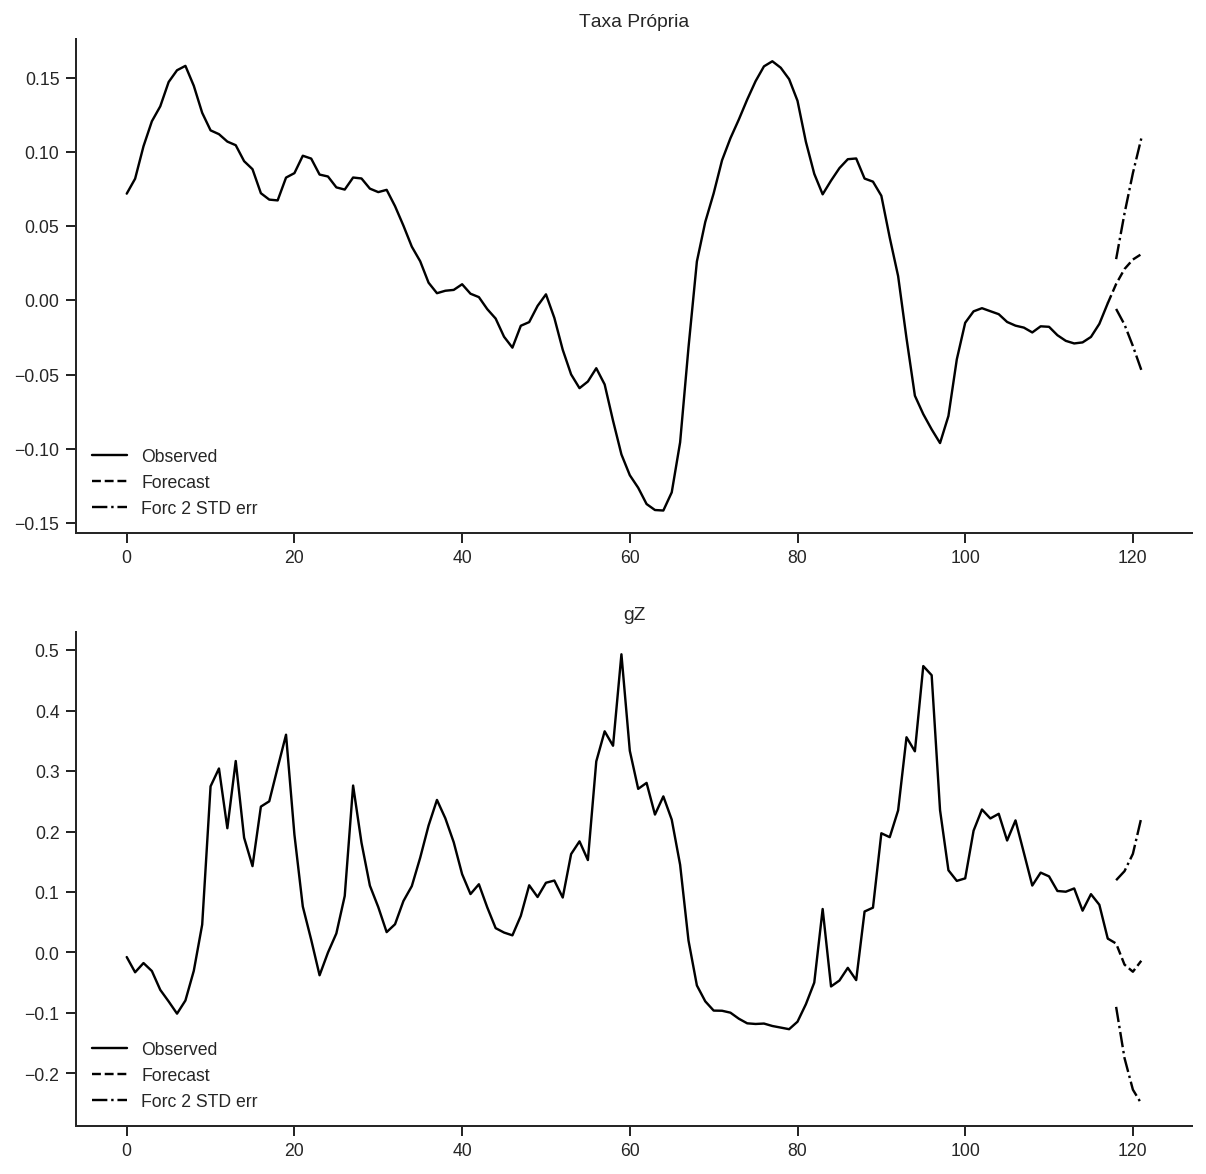
\includegraphics[width=\textwidth]{Fatos_Estilizados/Figs/Previsao_VECM.png}
	\caption*{\textbf{Fonte:} Elaboração própria}
\end{figure}


\begin{center}
\begin{table}[H]
\centering
\caption{Parâmetros para a equação da Taxa Própria}
\begin{tabular}{lccclcc}
\toprule
\textbf{Equação:} Taxa própria & \textbf{coef} & \textbf{std err} & \textbf{z} & \textbf{P$> |$z$|$} & \textbf{[0.025} & \textbf{0.975]}  \\
\midrule
\textbf{$L^1 $ Taxa Própria} &       0.9320  &        0.089     &    10.511  &         0.000***        &        0.758    &        1.106     \\
\textbf{$L^1 $ gZ}           &      -0.0545  &        0.014     &    -3.786  &         0.000***        &       -0.083    &       -0.026     \\
\textbf{$L^2 $ Taxa Própria} &      -0.2810  &        0.122     &    -2.305  &         0.021**        &       -0.520    &       -0.042     \\
\textbf{$L^2 $ gZ}           &       0.0040  &        0.013     &     0.309  &         0.758        &       -0.021    &        0.029     \\
\textbf{$L^3 $ Taxa Própria} &       0.0043  &        0.127     &     0.034  &         0.973        &       -0.245    &        0.253     \\
\textbf{$L^3 $ gZ}           &      -0.0132  &        0.012     &    -1.058  &         0.290        &       -0.038    &        0.011     \\
\textbf{$L^4 $ Taxa Própria} &      -0.0626  &        0.126     &    -0.497  &         0.619        &       -0.309    &        0.184     \\
\textbf{$L^4 $ gZ}           &      -0.0030  &        0.012     &    -0.242  &         0.809        &       -0.027    &        0.021     \\
\textbf{$L^5 $ Taxa Própria} &       0.0144  &        0.093     &     0.156  &         0.876        &       -0.167    &        0.196     \\
\textbf{EC1} &      -0.0099  &        0.007     &    -1.339  &         0.181        &       -0.024    &        0.005     \\
\textbf{$\beta_1$ } &       1.0000  &            0     &         0  &         0.000***        &        1.000    &        1.000     \\\bottomrule
\end{tabular}
\caption*{\textbf{Fonte:} Elaboração própria}
\end{table}
\end{center}

\begin{table}[H]
\begin{center}
\caption{Parâmetros para a equação da $g_{I_h}$}	
\begin{tabular}{lccclcc}
\toprule
\textbf{Equação:} $g_{I_h}$ & \textbf{coef} & \textbf{std err} & \textbf{z} & \textbf{P$> |$z$|$} & \textbf{[0.025} & \textbf{0.975]}  \\
\midrule
\textbf{$L^1 $ Taxa Própria} &      -0.8392  &        0.553     &    -1.517  &         0.129        &       -1.924    &        0.245     \\
\textbf{$L^1 $ gZ}           &       0.1290  &        0.090     &     1.435  &         0.151        &       -0.047    &        0.305     \\
\textbf{$L^2 $ Taxa Própria} &      -1.6629  &        0.761     &    -2.186  &         0.029**        &       -3.154    &       -0.172     \\
\textbf{$L^2 $ gZ}           &      -0.0663  &        0.081     &    -0.817  &         0.414        &       -0.225    &        0.093     \\
\textbf{$L^3 $ Taxa Própria} &       1.5635  &        0.793     &     1.972  &         0.049**        &        0.009    &        3.118     \\
\textbf{$L^3 $ gZ}           &       0.1092  &        0.078     &     1.407  &         0.159        &       -0.043    &        0.261     \\
\textbf{$L^4 $ Taxa Própria} &      -0.5929  &        0.785     &    -0.755  &         0.450        &       -2.132    &        0.946     \\
\textbf{$L^4 $ gZ}           &      -0.4590  &        0.078     &    -5.895  &         0.000***        &       -0.612    &       -0.306     \\
\textbf{$L^5 $ Taxa Própria} &      -0.3158  &        0.577     &    -0.547  &         0.584        &       -1.447    &        0.816     \\
\textbf{$L^5 $ gZ}           &       0.0265  &        0.089     &     0.299  &         0.765        &       -0.147    &        0.200     \\
\textbf{EC1} &       0.1388  &        0.046     &     3.021  &         0.003**        &        0.049    &        0.229     \\
\textbf{$\beta_2$ } &      -0.4833  &        0.230     &    -2.099  &         0.036**        &       -0.934    &       -0.032     \\\bottomrule
\end{tabular}
\caption*{\textbf{Fonte:} Elaboração própria}
\end{center}
\end{table}

\end{comment}
